%%%%%%%%%%%%%%%%%%%%%%%%%%%%%%%%%%%%%%%%%%%%%%%%%%%%
% Document type, global settings, and packages
%%%%%%%%%%%%%%%%%%%%%%%%%%%%%%%%%%%%%%%%%%%%%%%%%%%%

\PassOptionsToPackage{normalem}{ulem}
\documentclass[12pt]{report}   %12 point font for Times New Roman
\usepackage{graphicx}  %for images and plots
\usepackage[a4paper, left=1.5in, right=1in, top=1in, bottom=1in]{geometry}
\usepackage{setspace}  %use this package to set linespacing as desired
%\usepackage{times}  %set Times New Roman as the font
\usepackage{garamondx}
\usepackage{ebgaramond}\usepackage[ugm]{mathdesign}
\usepackage[explicit]{titlesec}  %title control and formatting
\usepackage[titles]{tocloft}  %table of contents control and formatting
\usepackage[backend=bibtex, sorting=none, bibstyle=ieee]{biblatex}  %reference manager
\usepackage[bookmarks=true, hidelinks]{hyperref}
\usepackage[page]{appendix}  %for appendices
\usepackage{rotating}  %for rotated, landscape images
\usepackage{ulem}  %for underlined section titles
\usepackage{xltxtra} %for undelines in text mode
\usepackage{gensymb,siunitx} %for temperature symbols
\usepackage{comment} %for radio tables
\usepackage{amsmath} %for align equations
\usepackage{ulem} %for underlined text
\usepackage{caption}
\usepackage{subcaption} %for matrix of figures
\usepackage{placeins} %for FloatBarrier

%%%%%%%%%%%%%%%%%%%%%%%%%%%%%%%%%%%
% Bibliography
%%%%%%%%%%%%%%%%%%%%%%%%%%%%%%%%%%% 

% Add your bibliography file here
\bibliography{Introduction}
\bibliography{Review}
\bibliography{WHR}
\bibliography{SplitCycle}
\bibliography{Model}

% prevent certain fields in references from printing in bibliography
\AtEveryBibitem{\clearfield{issn}}
\AtEveryBibitem{\clearlist{issn}}

\AtEveryBibitem{\clearfield{language}}
\AtEveryBibitem{\clearlist{language}}

\AtEveryBibitem{\clearfield{doi}}
\AtEveryBibitem{\clearlist{doi}}

\AtEveryBibitem{\clearfield{url}}
\AtEveryBibitem{\clearlist{url}}

\AtEveryBibitem{%
  \ifentrytype{online}
    {}
    {\clearfield{urlyear}\clearfield{urlmonth}\clearfield{urlday}}}
  
%%%%%%%%%%%%%%%%%%%%%%
% Start of Document
%%%%%%%%%%%%%%%%%%%%%%
  
\begin{document}
%\doublespacing  %set line spacing

%%%%%%%%%%%%%%%%%%%%%%%%%%%%%%%%%%%%%
% Title Page
%%%%%%%%%%%%%%%%%%%%%%%%%%%%%%%%%%%%%

%%%% Define your thesis title, your name, your school, and your month and year of graduation here

\newcommand{\thesisTitle}{A comparison study between different WHR methodologies}
\newcommand{\yourName}{Nicola Zanardi}
\newcommand{\yourSchool}{Energy Engineering}
\newcommand{\yourMonth}{July}
\newcommand{\yourYear}{2016}

%%%%%%%%%%%%%%%%%%%%%%%%%%%%%%%%%%%%%%%%%%%%%%%%%%%%%%%%%
% Do not edit these lines unless you wish to customize
% the template
%%%%%%%%%%%%%%%%%%%%%%%%%%%%%%%%%%%%%%%%%%%%%%%%%%%%%%%%%



\begin{titlepage}
\begin{center}
  
\begin{singlespacing}
  
\textbf{\MakeUppercase{\thesisTitle}}\\
\vspace{10\baselineskip}
A Dissertation\\
Presented to\\
The Academic Faculty\\
\vspace{3\baselineskip}
By\\
\vspace{3\baselineskip}
\yourName\\
\vspace{3\baselineskip}
In Partial Fulfillment\\
of the Requirements for the Degree\\
Doctor of Philosophy in the\\
School of \yourSchool\\
\vspace{3\baselineskip}
Politecnico di Milano\\
\vspace{\baselineskip}
\yourMonth{} \yourYear{}
\vfill
Copyright \copyright{} \yourName{} \yourYear{}

\end{singlespacing}

\end{center}
\end{titlepage}



%%\currentpdfbookmark{Title Page}{titlePage}  %add PDF bookmark for this page

%%%%%%%%%%%%%%%%%%%%%%%%%%%%%%%%%%%%%
% Approval Page
%%%%%%%%%%%%%%%%%%%%%%%%%%%%%%%%%%%%%

%%% Define your committee members. If you have less than 6, simple delete/comment the unused lines

\newcommand{\committeeMemberOne}{Prof. Onorati, Angelo}
\newcommand{\committeeMemberOneDepartment}{School of Energy Engineering}
\newcommand{\committeeMemberOneAffiliation}{Politecnico di Milano}

\newcommand{\committeeMemberTwo}{Prof. Canova, Marcello}
\newcommand{\committeeMemberTwoDepartment}{School of Mechanical Engineering}
\newcommand{\committeeMemberTwoAffiliation}{Ohio State University}

\newcommand{\committeeMemberThree}{Dr. Three}
\newcommand{\committeeMemberThreeDepartment}{School of Electrical Engineering}
\newcommand{\committeeMemberThreeAffiliation}{Georgia Institute of Technology}

\newcommand{\committeeMemberFour}{Dr. Four}
\newcommand{\committeeMemberFourDepartment}{School of Computer Science}
\newcommand{\committeeMemberFourAffiliation}{Georgia Institute of Technology}

\newcommand{\committeeMemberFive}{Dr. Five}
\newcommand{\committeeMemberFiveDepartment}{School of Public Policy}
\newcommand{\committeeMemberFiveAffiliation}{Georgia Institute of Technology}

\newcommand{\committeeMemberSix}{Dr. Six}
\newcommand{\committeeMemberSixDepartment}{School of Nuclear Engineering}
\newcommand{\committeeMemberSixAffiliation}{Georgia Institute of Technology}

\newcommand{\approvalDay}{11}
\newcommand{\approvalMonth}{July}
\newcommand{\approvalYear}{2016}

%%%%%%%%%%%%%%%%%%%%%%%%%%%%%%%%%%%%%%%%%%%%%%%%%%%%%%%%%
% Do not edit these lines unless you wish to customize
% the template
%%%%%%%%%%%%%%%%%%%%%%%%%%%%%%%%%%%%%%%%%%%%%%%%%%%%%%%%%


\begin{titlepage}
\begin{singlespacing}
\begin{center}
  
\textbf{\MakeUppercase{\thesisTitle}}\\
\vspace{10\baselineskip}

\end{center}
\vfill

%Define minipages, depending on how many authors there are
\ifdefined\committeeMemberFour

Approved by:
\vspace{2\baselineskip}		%adjust the number in front of "\baselineskip" for alignment

\begin{minipage}[b]{0.4\textwidth}
  
	\committeeMemberOne\\
	\committeeMemberOneDepartment\\
	\textit{\committeeMemberOneAffiliation}\\
	
	\committeeMemberTwo\\
	\committeeMemberTwoDepartment\\
	\textit{\committeeMemberTwoAffiliation}\\
	
	\committeeMemberThree\\
	\committeeMemberThreeDepartment\\
	\textit{\committeeMemberThreeAffiliation}\\
	
	\vspace{2\baselineskip}		%adjust the number in front of "\baselineskip" for alignment
	
\end{minipage}
\hspace{0.1\textwidth}
\begin{minipage}[b]{0.4\textwidth}
  
	\committeeMemberFour\\
	\committeeMemberFourDepartment\\
	\textit{\committeeMemberFourAffiliation}\\
	
	\ifdefined\committeeMemberSix
	\committeeMemberFive\\
	\committeeMemberFiveDepartment\\
	\textit{\committeeMemberFiveAffiliation}\\
	
	\committeeMemberSix\\
	\committeeMemberSixDepartment\\
	\textit{\committeeMemberSixAffiliation}\\
	
	Date Approved: \approvalMonth{} \approvalDay, \approvalYear
	\vspace{1\baselineskip}		%adjust the number in front of "\baselineskip" for alignment
	
	\else
	
	\committeeMemberFive\\
	\committeeMemberFiveDepartment\\
	\textit{\committeeMemberFiveAffiliation}\\
		
	Date Approved: \approvalMonth{} \approvalDay, \approvalYear
	\vspace{5\baselineskip}		%adjust the number in front of "\baselineskip" for alignment
	
	\fi
	
\end{minipage}

\else

\hspace{0.6\textwidth}
\begin{minipage}[b]{0.4\textwidth}
	
	Approved by:
	\vspace{2\baselineskip}		%adjust the number in front of "\baselineskip" for alignment
	
	\committeeMemberOne\\
	\committeeMemberOneDepartment\\
	\textit{\committeeMemberOneAffiliation}\\
	
	\committeeMemberTwo\\
	\committeeMemberTwoDepartment\\
	\textit{\committeeMemberTwoAffiliation}\\
	
	\committeeMemberThree\\
	\committeeMemberThreeDepartment\\
	\textit{\committeeMemberThreeAffiliation}\\
	
	\vspace{2\baselineskip}		%adjust the number in front of "\baselineskip" for alignment
	
	Date Approved: \approvalMonth{} \approvalDay, \approvalYear
	\vspace{\baselineskip}		%adjust the number in front of "\baselineskip" for alignment
	
\end{minipage}

\fi





\end{singlespacing}
\end{titlepage}


%%%%%%%%%%%%%%%%%%%%%%%%%%%%%%%%%%%%%
% Epigraph
%%%%%%%%%%%%%%%%%%%%%%%%%%%%%%%%%%%%%

%% Define your quote and author for the epigraph here

\newcommand{\yourQuote}{A great quote to start the thesis}
\newcommand{\yourAuthor}{George P. Burdell}

%%%%%%%%%%%%%%%%%%%%%%%%%%%%%%%%%%%%%%%%%%%%%%%%%%%%%%%%%
% Do not edit these lines unless you wish to customize
% the template
%%%%%%%%%%%%%%%%%%%%%%%%%%%%%%%%%%%%%%%%%%%%%%%%%%%%%%%%%

\begin{titlepage}
\begin{center}

\vspace*{\fill}
\yourQuote\\
\textit{\yourAuthor}
\vspace*{\fill}

\end{center}
\end{titlepage}



%%%%%%%%%%%%%%%%%%%%%%%%%%%%%%%%%%%%%
% Dedication
%%%%%%%%%%%%%%%%%%%%%%%%%%%%%%%%%%%%%

%% Define your dedication statement here

\newcommand{\yourDedication}{A great dedication goes here.}

%%%%%%%%%%%%%%%%%%%%%%%%%%%%%%%%%%%%%%%%%%%%%%%%%%%%%%%%%
% Do not edit these lines unless you wish to customize
% the template
%%%%%%%%%%%%%%%%%%%%%%%%%%%%%%%%%%%%%%%%%%%%%%%%%%%%%%%%%

\begin{titlepage}
\begin{center}

\vspace*{\fill}
\yourDedication\\
\vspace*{\fill}

\end{center}
\end{titlepage}


%%%%%%%%%%%%%%%%%%%%%%%%%%%%%%%%%%%%%
% Acknowledgments
%%%%%%%%%%%%%%%%%%%%%%%%%%%%%%%%%%%%%

\pagenumbering{roman}
\addcontentsline{toc}{chapter}{Acknowledgments}
\setcounter{page}{5} % set the page number appropriately based on the number of intro pages
%\clearpage
\begin{centering}
\textbf{ACKNOWLEDGEMENTS}\\
\vspace{\baselineskip}
\end{centering}

%Insert your dedication text here
Lorem ipsum dolor sit amet, consectetur adipiscing elit, sed do eiusmod tempor incididunt ut labore et dolore magna aliqua. Ut enim ad minim veniam, quis nostrud exercitation ullamco laboris nisi ut aliquip ex ea commodo consequat. Duis aute irure dolor in reprehenderit in voluptate velit esse cillum dolore eu fugiat nulla pariatur. Excepteur sint occaecat cupidatat non proident, sunt in culpa qui officia deserunt mollit anim id est laborum.

\clearpage
%\pagenumbering{gobble}  %remove page number on summary page


%\addtocontents{toc}{\cftpagenumbersoff{chapter}} 

%\currentpdfbookmark{Acknowledgments}{acknowledgments}
%\addtocontents{toc}{\cftpagenumberson{chapter}} 

%%%%%%%%%%%%%%%%%%%%%%%%%%%%%%%%%%%%%
% Table of Contents
%%%%%%%%%%%%%%%%%%%%%%%%%%%%%%%%%%%%%

% Format for Table of Contents
\renewcommand{\cftchapdotsep}{\cftdotsep}  %add dot separators
\renewcommand{\cftchapfont}{\bfseries}  %set title font weight
\renewcommand{\cftchappagefont}{}  %set page number font weight
\renewcommand{\cftchappresnum}{Chapter }
\renewcommand{\cftchapaftersnum}{:}
\renewcommand{\cftchapnumwidth}{5em}
\renewcommand{\cftchapafterpnum}{\vskip\baselineskip} %set correct spacing for entries in single space environment
\renewcommand{\cftsecafterpnum}{\vskip\baselineskip}  %set correct spacing for entries in single space environment
\renewcommand{\cftsubsecafterpnum}{\vskip\baselineskip} %set correct spacing for entries in single space environment
\renewcommand{\cftsubsubsecafterpnum}{\vskip\baselineskip} %set correct spacing for entries in single space environment

%format title font size and position (this also applys to list of figures and list of tables)
\titleformat{\chapter}[display]
{\normalfont\bfseries\filcenter}{\chaptertitlename\ \thechapter}{0pt}{\MakeUppercase{#1}}

\renewcommand\contentsname{Table of Contents}

\begin{singlespace}
\tableofcontents
\end{singlespace}

\currentpdfbookmark{Table of Contents}{TOC}

\clearpage

%%%%%%%%%%%%%%%%%%%%%%%%%%%%%%%%%%%%%
% List of figures and tables
%%%%%%%%%%%%%%%%%%%%%%%%%%%%%%%%%%%%%

\addcontentsline{toc}{chapter}{List of Tables}
\begin{singlespace}
	\setlength\cftbeforetabskip{\baselineskip}  %manually set spacing between entries
	\listoftables
\end{singlespace}

\clearpage

\addcontentsline{toc}{chapter}{List of Figures}
\begin{singlespace}
\setlength\cftbeforefigskip{\baselineskip}  %manually set spacing between entries
\listoffigures
\end{singlespace}

\clearpage

%%%%%%%%%%%%%%%%%%%%%%%%%%%%%%%%%%%%%%%%%%%%%%%%%%%%%%%%%%%%%%%%%
% This is the Summary (abstract should be separate document)
%%%%%%%%%%%%%%%%%%%%%%%%%%%%%%%%%%%%%%%%%%%%%%%%%%%%%%%%%%%%%%%%%

%\clearpage
\begin{centering}
\textbf{SUMMARY}\\
\vspace{\baselineskip}
\end{centering}

Lorem ipsum dolor sit amet, consectetur adipiscing elit, sed do eiusmod tempor incididunt ut labore et dolore magna aliqua. Ut enim ad minim veniam, quis nostrud exercitation ullamco laboris nisi ut aliquip ex ea commodo consequat. Duis aute irure dolor in reprehenderit in voluptate velit esse cillum dolore eu fugiat nulla pariatur. Excepteur sint occaecat cupidatat non proident, sunt in culpa qui officia deserunt mollit anim id est laborum.

%\pagenumbering{gobble}  %remove page number on summary page

%%%%%%%%%%%%%%%%%%%%%%%%%%%%
%
% Chapters
%
%%%%%%%%%%%%%%%%%%%%%%%%%%%%

%%%%%%%%%%%%%%%%%%%%%%
% formatting
%%%%%%%%%%%%%%%%%%%%%%

% resume page numbering for rest of document
\clearpage
\pagenumbering{arabic}
\setcounter{page}{1} % set the page number appropriately

% Adjust chapter title formatting
\titleformat{\chapter}[display]
{\normalfont\bfseries\filcenter}{\MakeUppercase\chaptertitlename\ \thechapter}{0pt}{\MakeUppercase{#1}}  %spacing between titles
\titlespacing*{\chapter}
  {0pt}{0pt}{30pt}	%controls vertical margins on title
  
% Adjust section title formatting
\titleformat{\section}{\normalfont\bfseries}{\thesection}{1em}{#1}

% Adjust subsection title formatting
\titleformat{\subsection}{\normalfont}{\uline{\thesubsection}}{0em}{\uline{\hspace{1em}#1}}

% Adjust subsubsection title formatting
\titleformat{\subsubsection}{\normalfont\itshape}{\thesubsection}{1em}{#1}

%%%%%%%%%%%%%%%%
% Chapter 1
%%%%%%%%%%%%%%%%

\chapter{Introduction and Background}

The focus on reduction of greenhouse emissions from fossil fuels is today as important as ever. The rapid ongoing modifications of climate conditions are raising concerns and awareness in this regard. Total anthropogenic greenhouse emissions have continued to increase over 1970 to 2010, with larger absolute increase per decade toward the end of this period, with CO\textsubscript{2} emissions from fossil fuel combustion and industrial processes contributing about 78\% of the total. Annual anthropogenic GHG emissions have increased by 10 Gtons equivalent of CO2 between 2000 and 2010, with this increase directly coming from energy supply (47\%), industry (30\%), transport (11\%) and buildings (3\%) sectors \cite{IPCC2014}.

Global warming causes adverse effect and mutations on natural habitats and natural equilibriums of Earth, and is held responsible for increase of atmospheric temperature, acidification of oceans, melting of the permafrost, increased frequency of extreme weather events and others. As a result, many species struggle to adapt to these new environmental conditions and some are facing extinction. Even human related activities are in danger, as the natural habitat become more and more hostile to plants and animals. In the following sections the phenomenon will be explained in more details, and the role of transportation sector will be highlighted.

\section{Global warming and role of transport section emissions} \label{sec:global_warming}

\emph{Global warming} and \emph{Climate change} are terms used for describing the increase in surface and ocean temperature registered in the last century. Due to the accumulation of greenhouse gases, additional energy is stored in the atmosphere and the oceans, causing ice melting and warming of continents and atmosphere. 

\begin{figure}[h]
  \centering
  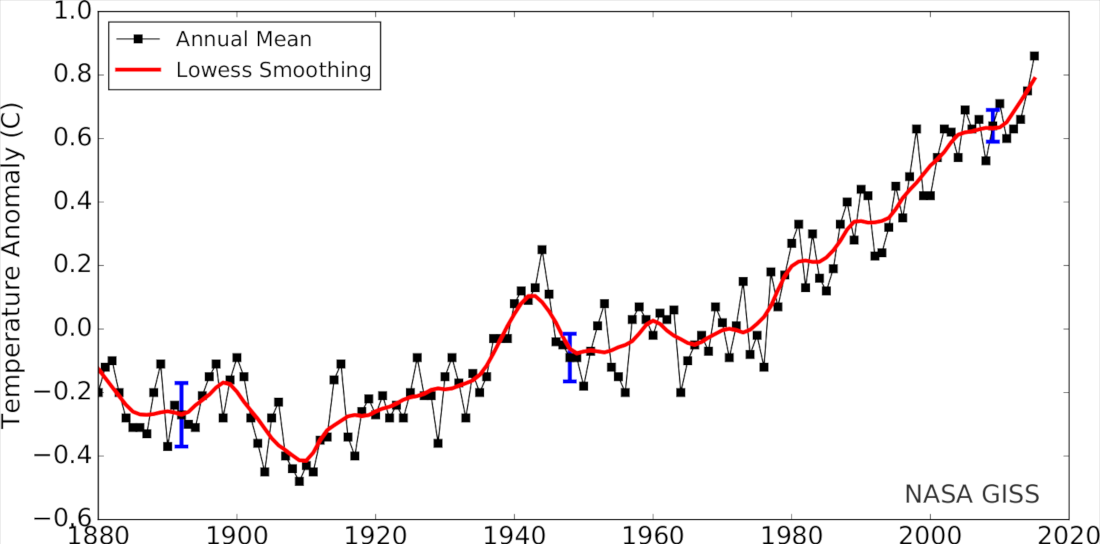
\includegraphics[width=0.8\textwidth]{figures/introduction/temp_rise.pdf}
  \caption{Global mean temperature estiamates based on land and ocean data\cite{GISS2016}}
  \label{antropogenic_ghg_emissions}
\end{figure}

Without additional efforts to reduce GHG emissions beyond those in place today, emissions growth is expected to persist driven by growth in global population and economic activities. Baseline scenarios, those without additional mitigation, result in global mean surface temperature increases in 2100 from \SI{3.7}{\celsius} to \SI{4.8}{\celsius} compared to pre-industrial levels \cite{IPCC2014}. Of the 49 Gt CO\textsubscript{2,eq} emitted in 2010, the \emph{transportation} sector is responsible for 14.3\% of the total, ranking as the fourth major emitter economic sector after Electricity and Heat production, Agriculture and Land use, and Industry.

\begin{figure}[h]
  \centering
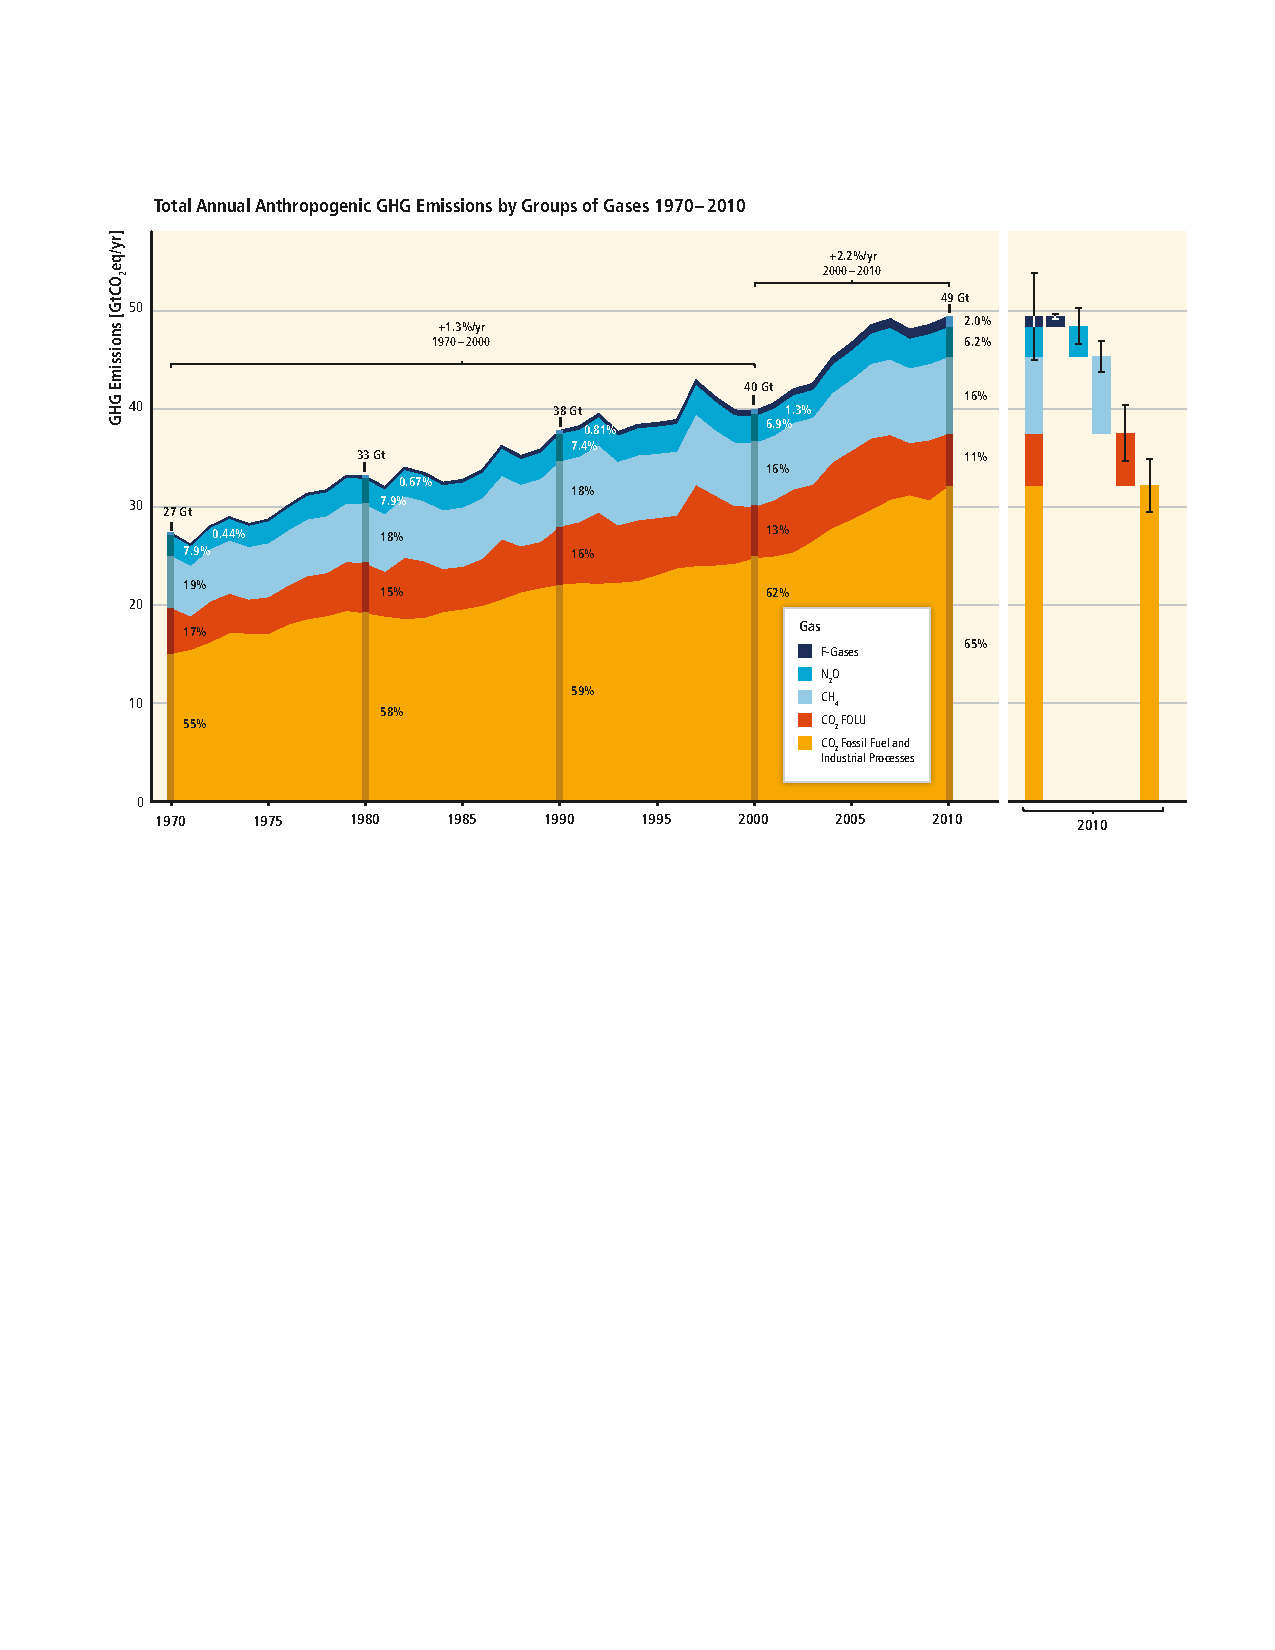
\includegraphics[width=0.8\textwidth]{figures/introduction/antropogenic_ghg_emissions.pdf}
  \caption{Antropogenic GHG emissions by group of gases (1970 - 2010) \cite{IPCC2014}}
  \label{antropogenic_ghg_emissions}
\end{figure}

The scientific community mainly agrees on trying to keep the temperature increase with respect to pre-industrial levels under \SI{2}{\celsius}, equivalent to atmospheric concentrations in 2100 of about 450 ppm CO\textsubscript{2,eq}. The aforementioned scenarios include substantial cuts in anthropogenic GHG emissions by mid century through large scale changes in energy systems and potentially land use. Scenarios reaching these concentrations by 2100 are characterized by lower global GHG emissions in 2050 than in 2010, 40\% to 70\% lower globally, and emissions levels near zero Gt CO\textsubscript{2,eq} or below in 2100 \cite{IPCC2014}. In Figure \ref{fig:mitigationscenarios}, the reduction in emissions for the major economic sectors is reported. It's possible to notice how, especially in the case without heavy implementation of carbon dioxide capture plants, the amount of greenhouse gases released in the atmosphere by transport must be greatly reduced.

\begin{figure}[ht]
  \centering
  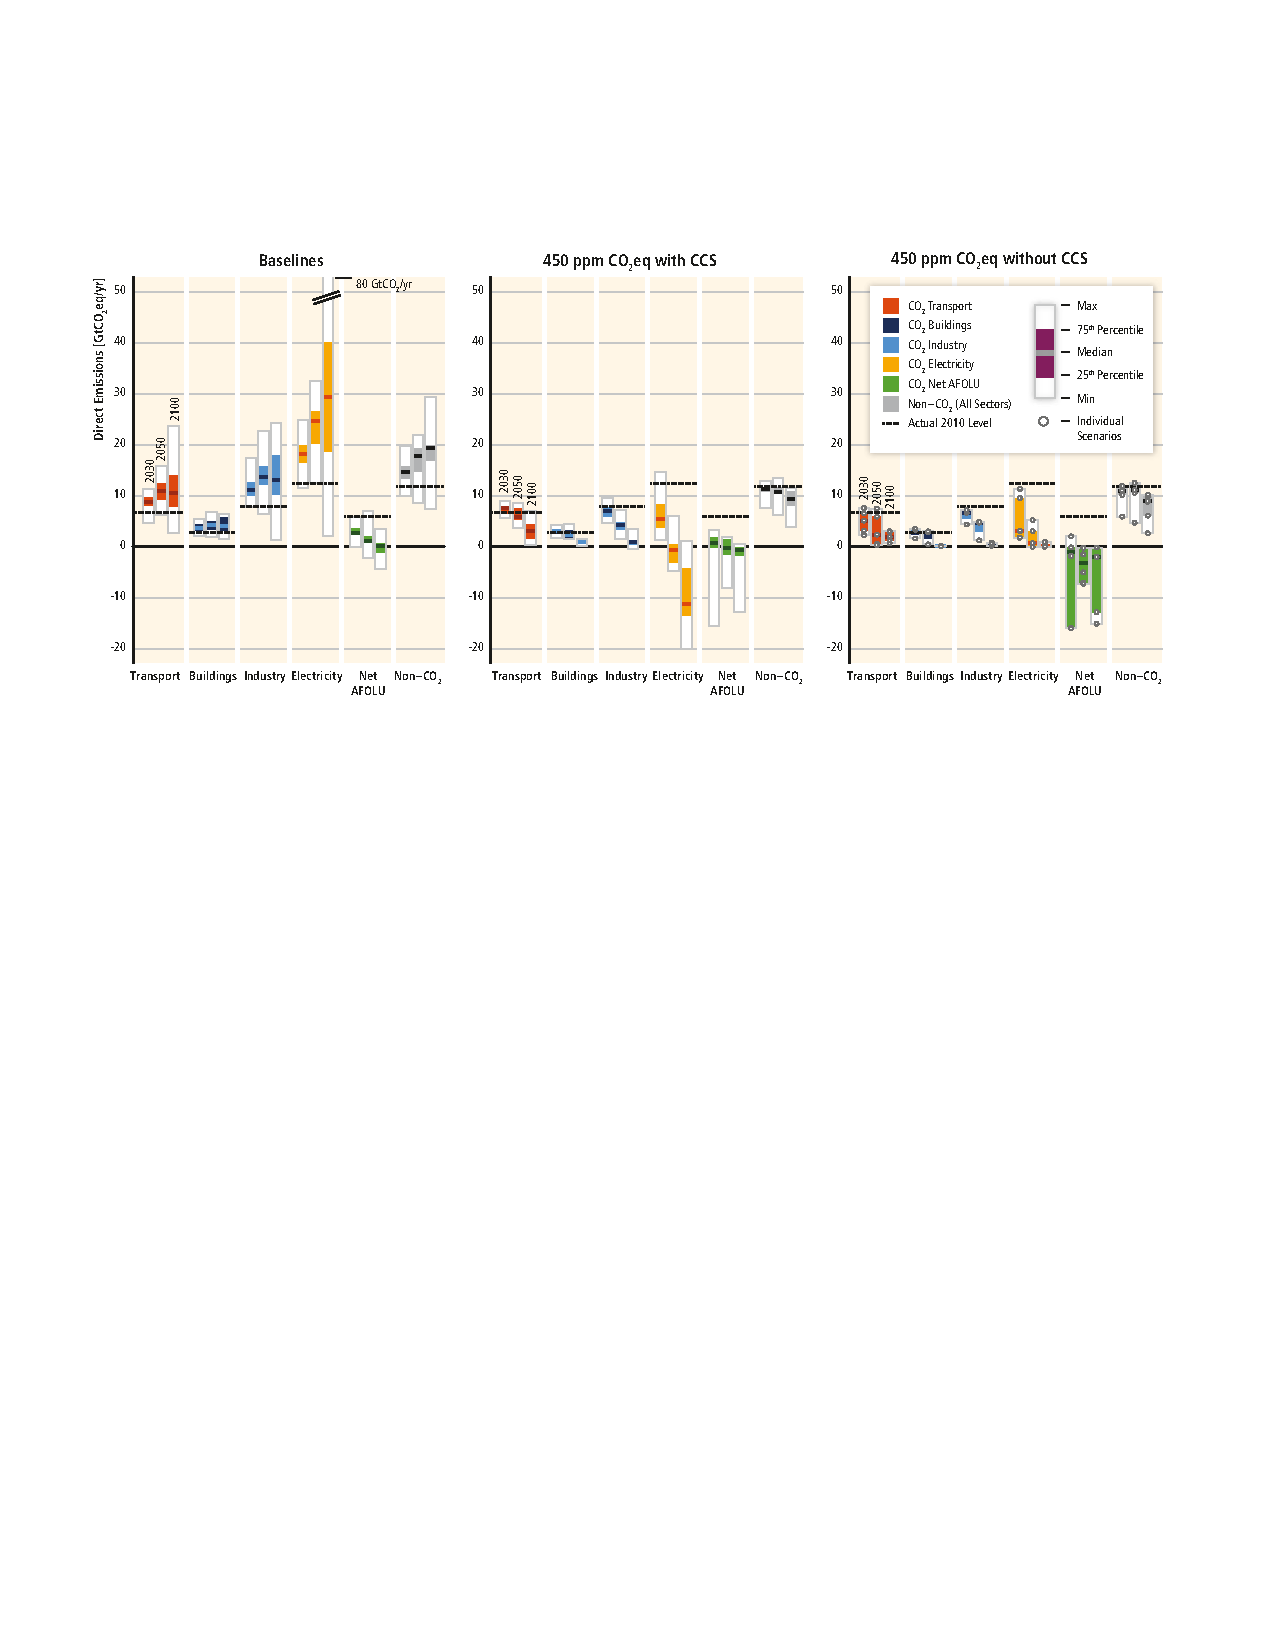
\includegraphics[width=\textwidth]{figures/introduction/mitigation_scenarios.pdf}
  \caption{Review of different mitigation scenarios for 450 ppm \label{fig:mitigationscenarios}}
\end{figure}

The chart represents a review of the major models and scenarios available to date, and taken into consideration in \cite{IPCC2014}. According to the same study, efficiency enhancements and behavioural changes aimed at reducing energy demand compared to baseline scenarios without compromising development, are a key mitigation strategy in scenarios reaching atmospheric CO\textsubscript{2,eq} concentrations of about 450 to about 500 ppm by 2100.

The transport sector accounted for 27\% of final energy use and 6.7 Gt CO\textsubscript{2} direct emissions in 2010, with baseline CO\textsubscript{2} emissions projected to approximately double by 2050. Technical and behavioural mitigation measures for all transport modes, plus new infrastructure and urban redevelopment investments, could reduce final energy demand in 2050 by around 40\% below the baseline \cite{IPCC2014}.

A study by Unger and al.~\cite{Unger2010} attributes a radiative forcing value to different economic sectors that are the main emitters in today economy. The radiative forcing concept has been developed in order to quantify the human and natural influence on the climate system, and is defined as the net energy flux difference at the top of the atmosphere. In Figure~\ref{fig:radiative_forcing}, the positive and negative contributions of the different economic sectors are presented. It's important to notice how on-road transportation is foreseen to be the major responsible for increasing of atmospheric energy content in 2020, and the second most important factor in 2100. This is due to the peculiar composition of exhaust gases produced by vehicles: the production is  mainly constituted by components that contribute to trapping heat. Other sectors, as the power sector, produce much more components that trap heat, but the net contribution is reduced by the amount of components as black-carbon, that reflects the solar radiation and contribute to cooling down the atmosphere. 

\begin{figure}[ht]
  \centering
  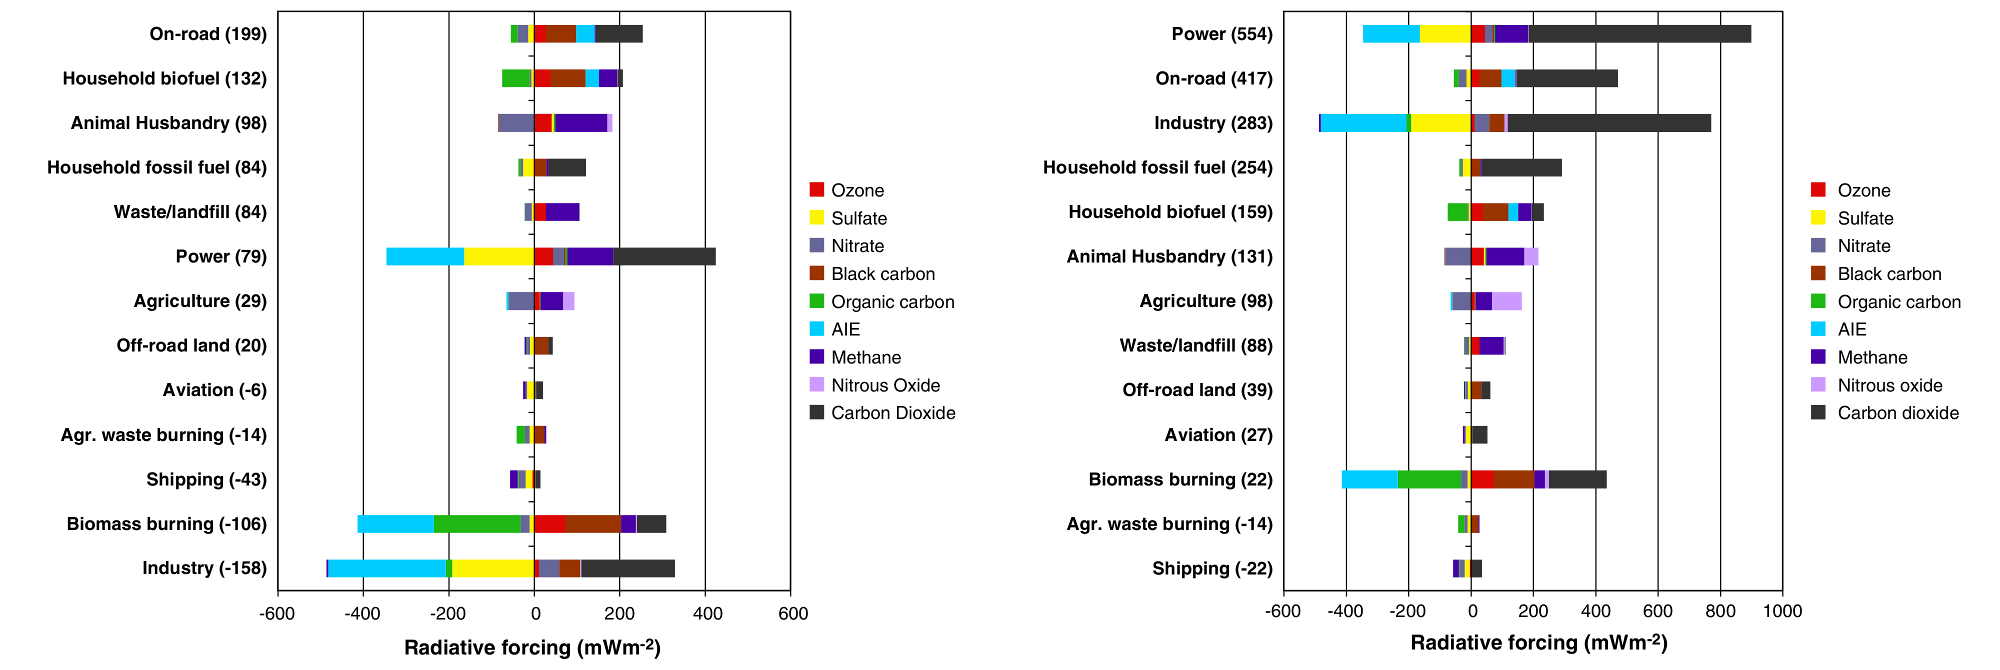
\includegraphics[width=\textwidth]{figures/introduction/radiative_forcing.png}
  \caption{Radiative forcing due to 2000 level emissions grouped by sector in a) 2020 and b) 2100 \label{fig:radiative_forcing}}
\end{figure}

\section{Current transportation scenario}

The average efficiency of modern internal combustion engines is measured to be around 32\% - 36\% for Diesel engines, and around 29\% - 32\% for Gasoline engines.

According to the evidence reported in section~\ref{sec:global_warming}, being the transportation sector one of the main culprits for global warming, an increase in efficiency of passenger vehicles can play an important role in mitigating climate change. Figure~\ref{fig:average_fuel_efficiency} shows how, in the 1980 - 2014 considered timeframe, the specific fuel consumption of U.S. vehicles has been reduced thanks to technical advancements~\cite{BureauofTransportationStatistics2016}.

\begin{figure}[ht]
  \centering
  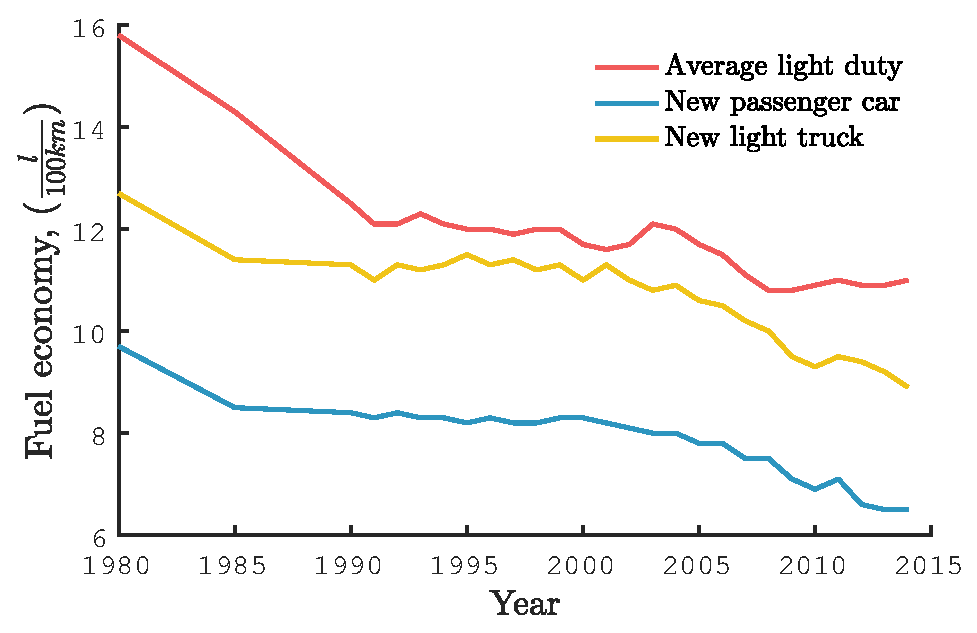
\includegraphics[width=0.8\textwidth]{figures/introduction/average_fuel_efficiency.eps}
  \caption{Average fuel efficiency for U.S. vehicles \label{fig:average_fuel_efficiency} }
\end{figure}

Taking a more in depth look at the emissions figure of the transportation economy itself, when considering the energy use by transportation mode in 2013, Highwway is by far the sector that consumes the greater share of the total (83.2\%), followed by Air transportation (6.9\%) and Water transportation (3.9\%). The Highway energy usage can be once again split between Light-duty (52.2\%), Combination Truck (15.3\%), Single-unit truck (7.6\%), and Bus (1.1\%). Certified air carriers experienced the largest total decrease in fuel consumption, consuming about 3.6 billion fewer gallons of jet fuel in 2014 than in 2000. General aviation gasoline showed the largest percent decrease in fuel consumption from 2000 to 2014, declining by 40.8 percent. Additionally, water modes powered by residual fuel oil also showed a large decrease, declining by nearly 2.6 billion gallons during the same period. Consistent with increases in vehicle-miles traveled, light-duty highway vehicles used about 430 million more gallons of gasoline in 2014 than in 2000~\cite{BureauofTransportationStatistics2016a}.

According to the evidence shown, the amount of effort spent on researching and experimenting new and more advanced ways of reducing transportation energy consumption is justified. Numerous different technical trends are nowadays gaining traction in the automotive field, such as downsizing and turbocharging of gasoline engines, or the usage of different cycles. A more in depth analysis will be provided in Section~\ref{sec:technology_improvements}.

\section{Evolution in internal combustion engines technology and efficiency}

In this section a review of the key technical improvements occurred to internal combustion engines in the last decades is presented, among with a brief explanation of the current emission limitation rules for both the USA and Europe. The final section will cover the importance of \emph{Waste Heat Recovery} (WHR) and why it needs to be researched and adopted in the next years in order to achieve the planned emissions limitation objectives.

\subsection{Improvements on overall engine efficiency in the last decades}

Since the petroleum crysis of the '70s, an increasing effort on reduction of fuel consumption and increase of power density has begun.

\begin{figure}[ht]
  \centering
  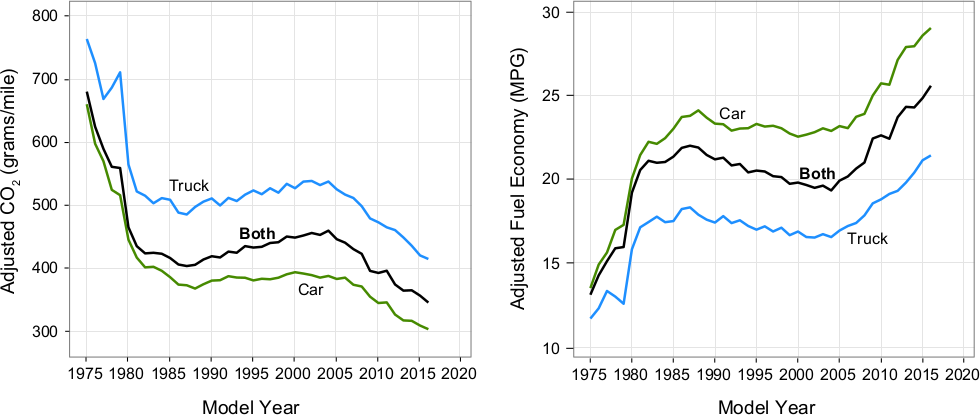
\includegraphics[width=\textwidth]{figures/review/adj_fuel_economy.pdf}
  \caption{Adjusted CO\textsubscript{2} and fuel economy for vehicles model year from 1975 to 2016\label{fig:adj_fuel_economy} }
\end{figure}

As shown in Figure~\ref{fig:adj_fuel_economy}~\cite{EPA2016}, during the last four decades, the fuel consumption and carbon dioxide emissions has been vastly reduced. This great improvement has been possible thanks to some key technical turning points.

One of the main design aspects that have changed significantly over time is how the fuel is delivered into the engine. Until the early 1980s the majority of engines used carburetors to meter fuel delivered to the combustion chamber. More recently, engines with gasoline direct injection (GDI) have begun to replace engines with port fuel injection. GDI equipped engines were first introduced with very limited production in Model Year (MY) 2007. Eight years later GDI engines were installed in about 42\% of MY 2015 vehicles, and are projected to achieve a 49\% market share in MY 2016~\cite{EPA2016}.

Another key aspect of engine design that has been vastly improved is the valve-train. The number of valves per cylinder and the ability to alter valve timing during the combustion cycle allowed significant power and efficiency improvements, as nowadays almost the entire fleet of the most relevant car manufacturers has converted to multi-valve design. While some three and five valve engines have been produced, the vast majority of multi-valve engines are based on four valves per cylinder~\cite{EPA2016}. In addition to the number of valves per cylinder, designs have evolved that allow engine valves to vary the timing when they are opened or closed with respect to the combustion cycle, creating more flexibility to control engine efficiency, power, and emissions. In Figure~\ref{fig:improvement_valve_fuel_delivery}, the fuel consumption reduction made possible by the improved valve-train and fuel delivery is shown. 

\begin{figure}[ht]
  \centering
  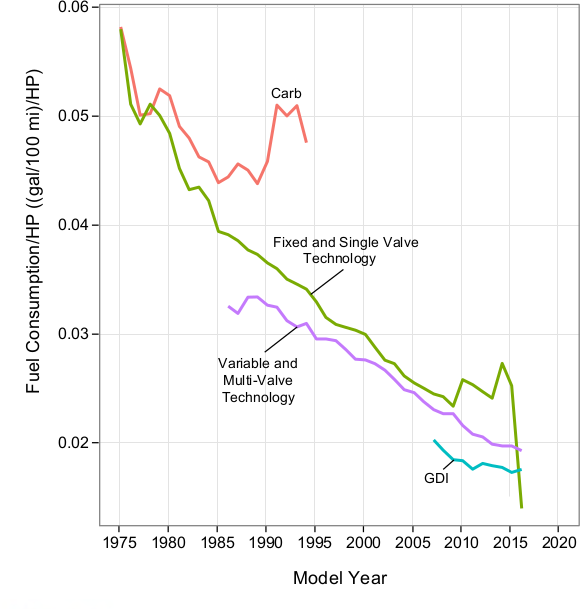
\includegraphics[width=0.7\textwidth]{figures/review/improvement_valve_fuel_delivery.pdf}
  \caption{Trends of fuel consumption variation with the introduction of major fuel delivery and valve-train control technologies \label{fig:improvement_valve_fuel_delivery} }
\end{figure}

As a result of the new fuel delivery systems, along with other reasons, two very noticeable trends in horsepower and displacement delineated. Average horsepower climbed consistently from MY 1982 to MY 2008. Since MY 2008, horsepower trends have been less consistent, and may be beginning to flatten out. From MY 1975 to 1987, the average engine displacement of new vehicles dropped dramatically by nearly 40 \%. From MY 1988 to 2004, displacement generally grew slowly, but the trend reversed in 2005 and engine displacement has been generally decreasing since. In MY 2016, engine displacement is projected to reach the lowest point on record, below the previous lowest average displacement reached in MY 1987~\cite{EPA2016}.

The contrasting trends in horsepower increase and displacement decrease are a proof of the continued improvements in engine design and of the impact of new technologies. The final result is a steady quasi-linear increase of the power density from around 0.5~$\frac{HP}{Displacement}$ in 1975 to around 1.4~$\frac{HP}{Displacement}$ in 2016, with a growth rate of 0.02~$\frac{HP}{in^{2} \cdot year}$. Also the average number of cylinders has gradually reduced.

In Figure~\ref{fig:technology_trends}, a summary of the time trends of the major innovations is reported.

\begin{figure}[ht]
  \centering  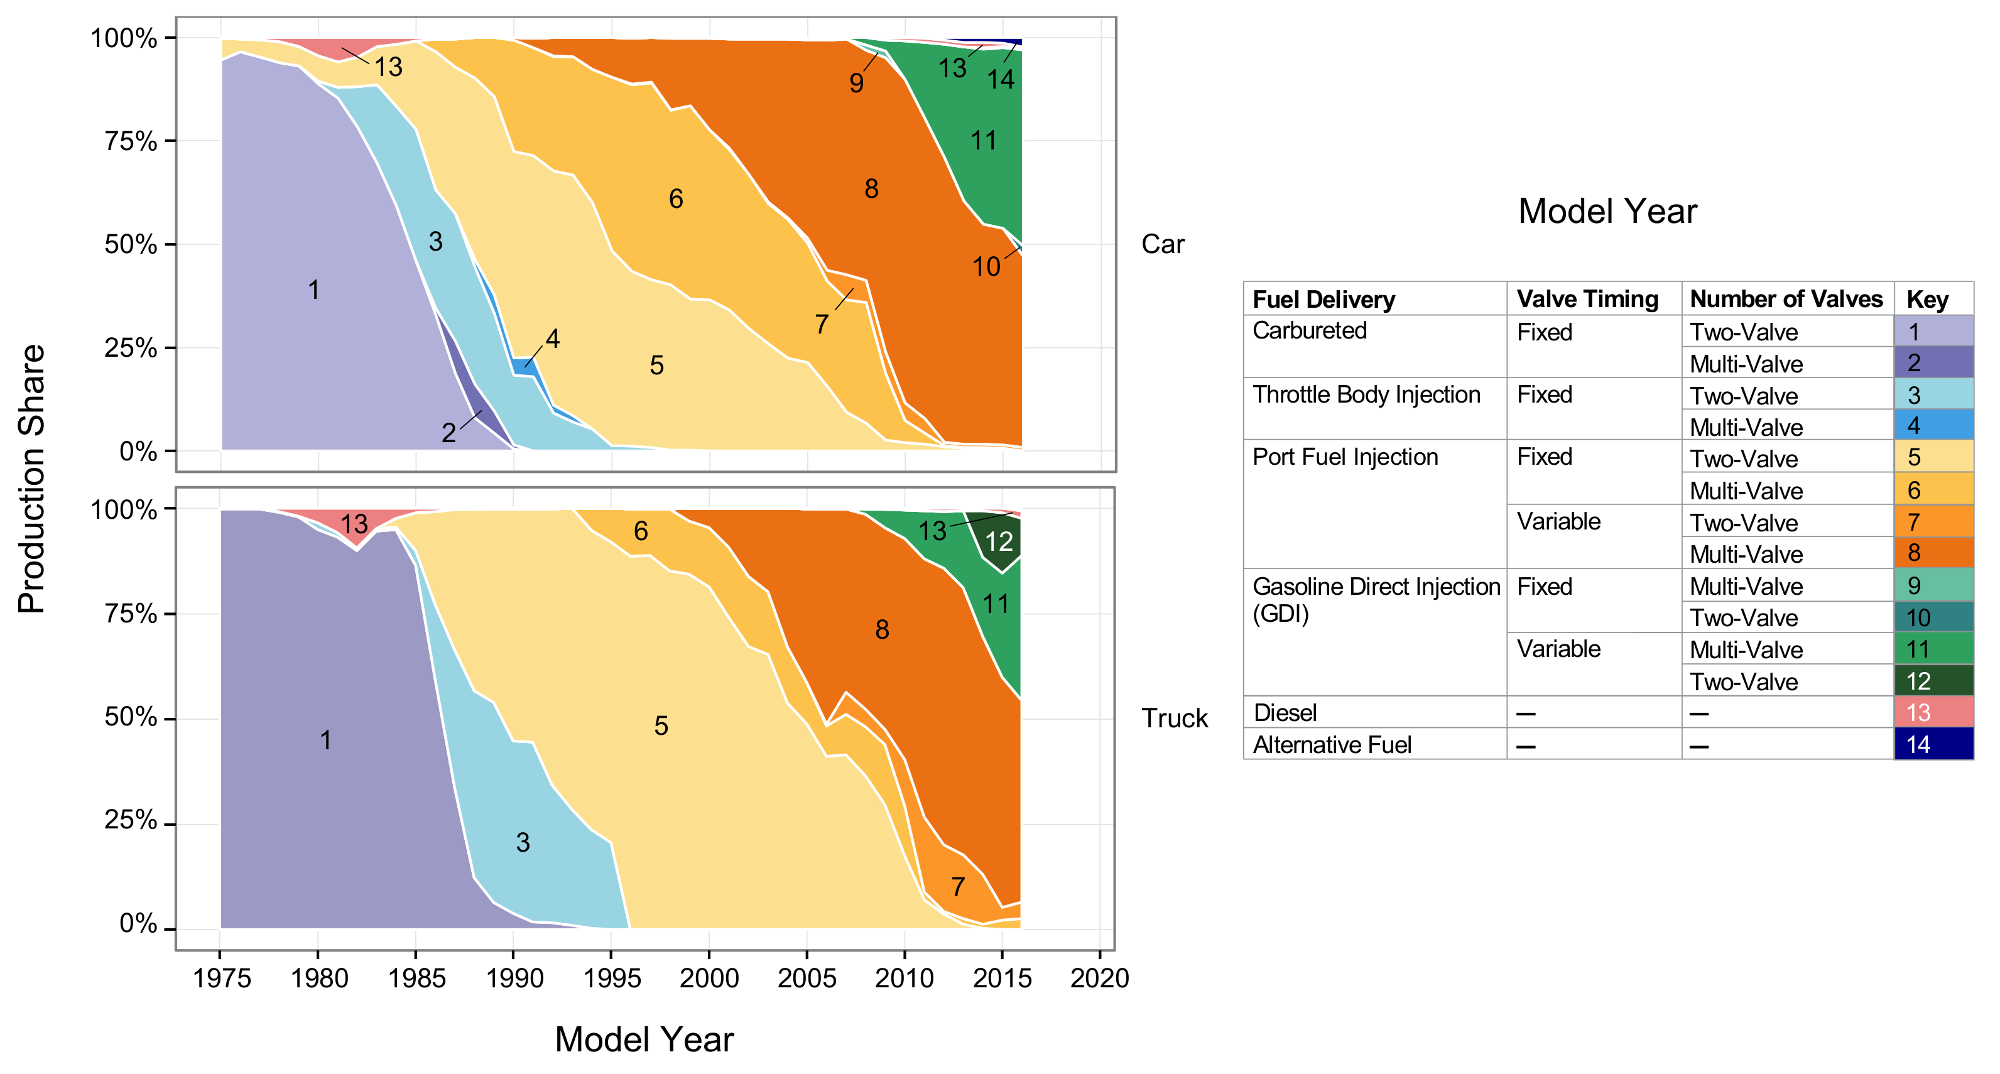
\includegraphics[width=\textwidth]{figures/review/technology_trends.png}
  \caption{Percentage of MY equipped with a certain technology  \label{fig:technology_trends} }
\end{figure}


\subsection{Emission limitations and trends in nowadays technology improvement}
\label{sec:technology_improvements}

Emission limitations are among the main drivers that fostered the continuous strive of greater efficiency in internal combustion engines. In Figure~\ref{fig:emission_standards} a review of the most important emissions standards from across the world, and their Euro equivalence is presented~\cite{Miller2014}. In Figure~\ref{fig:emission_levels} are reported the emission limits for gasoline and diesel powered light vehicles in both USA and Europe~\cite{Transportpolicy.net2016}.

\begin{figure}[ht]
  \centering
  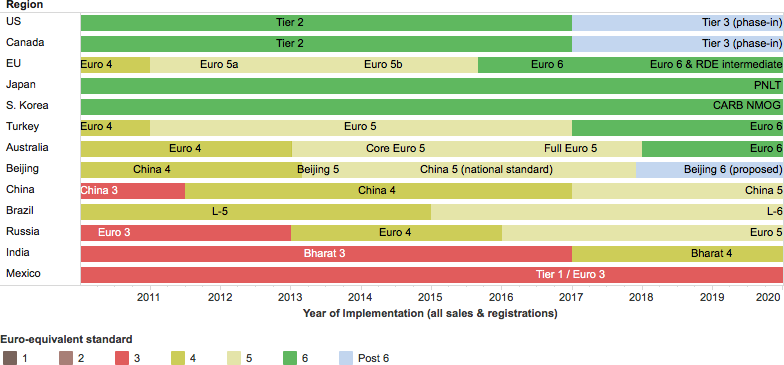
\includegraphics[width=\textwidth]{figures/review/emission_standards.png}
  \caption{Comparison of emissions standards with reference to Euro standards\label{fig:emission_standards} }
\end{figure}

\begin{figure}[ht]
  \centering
  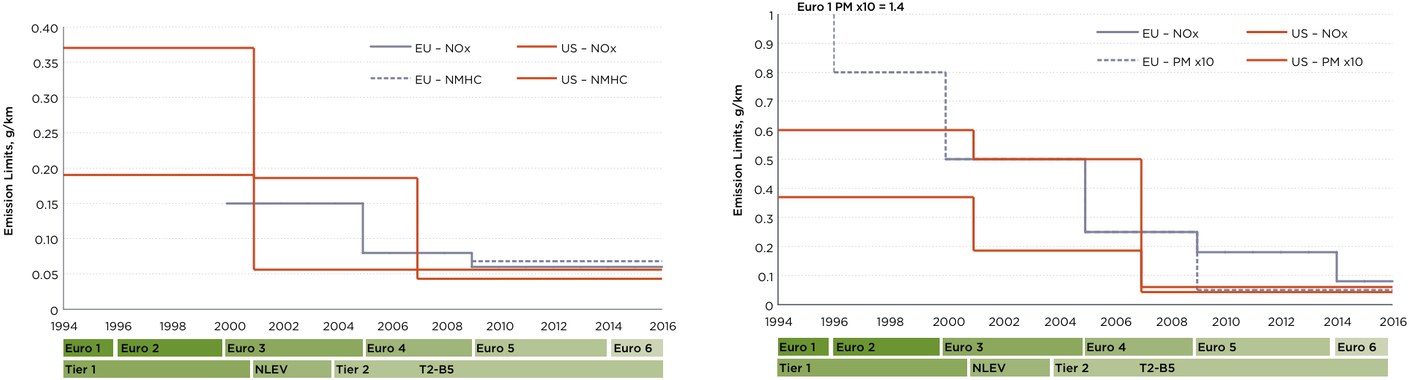
\includegraphics[width=\textwidth]{figures/review/emissions_levels.png}
  \caption{Emissions limits for a) Gasoline and b) Diesel light vehicles in USA and Europe\label{fig:emission_levels} }
\end{figure}

In order to respect the emission standards imposed by current and future rules, the major car manufacturers are adopting new technologies, and some trends are delineating. 

Probably the most noticeable trend in new engines is the \emph{turbo-downsizing}. This new group of engines is characterized usually by a similar power output with respect to the engine that are replacing, but a smaller displacement. This result is achieved by the introduction of turbochargers and, often but not always, GDI. Turbo downsized engines are an approach to engine design that provides increased fuel economy by using a smaller engine for most vehicle operation, while retaining the ability to provide more power via the turbocharger, when needed. Turbocharged engines are projected to constitute 22\% of new vehicle production in 2016, and the penetration trend appears to increase rapidly~\cite{EPA2016}. This is due to the fact the traditionally turbocharged engines were mainly used in high performance vehicles, while now they are being used also on mainstream vehicles. The increased power density and torque made available by the adoption of the turbocharger allows the shifting to designs with fewer cylinders, while the combination with GDI allows a more efficient engine operation and increases the resistance to knocking. In MY 2016, more than 90\% of new vehicles with gasoline turbocharged engines also use GDI~\cite{EPA2016}. In Figure~\ref{fig:turbodownsizing_distribution}, the distribution of gasoline turbo vehicles is shown. Other new technologies that are gaining traction in the engine design environment are Cylinder Deactivation, Non-Hybrid Stop/Start, and more advanced transmissions, both in form of transmissions with seven or more gears or Continuous-Variable Transmissions (CVT).

\begin{figure}[ht]
  \centering
  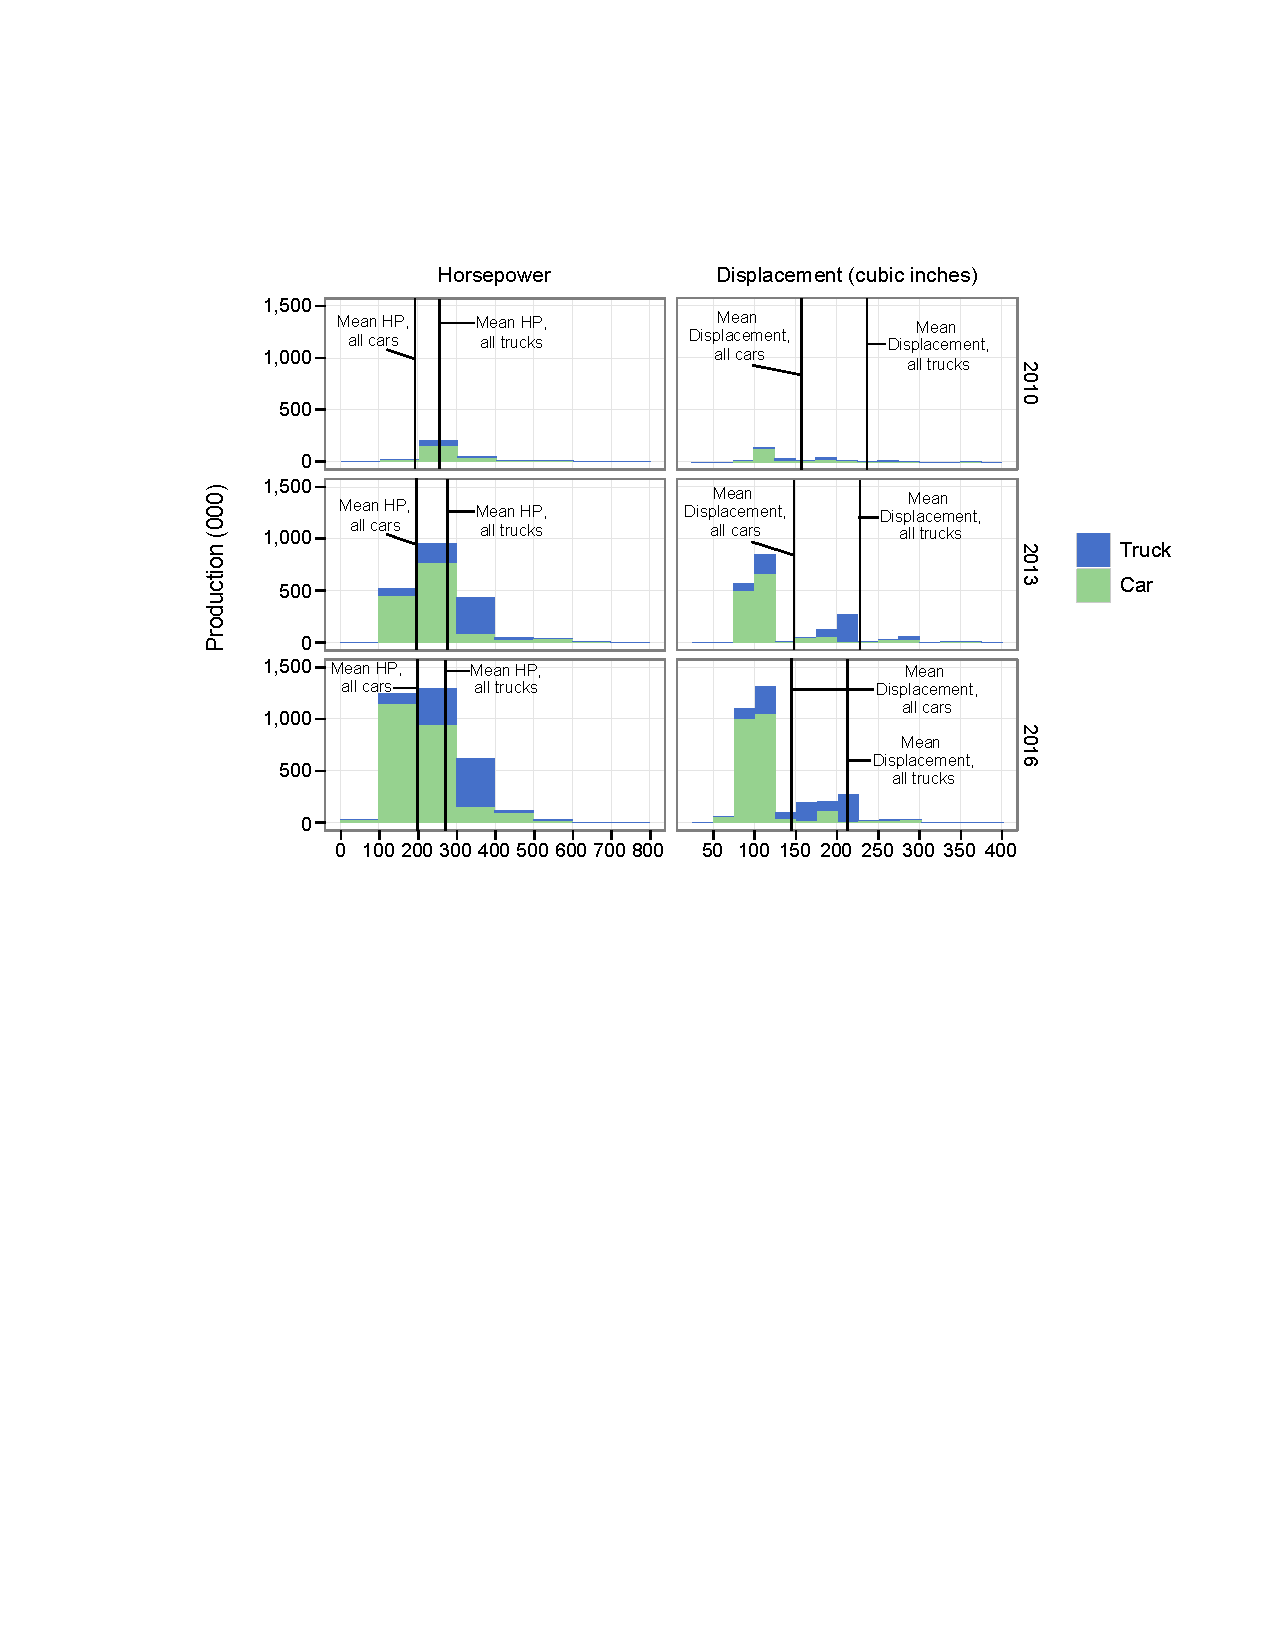
\includegraphics[width=0.8\textwidth]{figures/review/turbodownsizing_distribution.pdf}
  \caption{Distribution of Gasoline Turbo Vehicles by Displacement and Horsepower, MY 2010, 2013, and 2016\label{fig:turbodownsizing_distribution} }
\end{figure}



\emph{Hybrid} vehicle technology is the most diffused technique used to increase the fuel efficiency in ways that transcend the pure ICE efficiency increase. Hybrid vehicles utilize larger battery packs, electric motors, and other components that can  increase vehicle fuel economy. Benefits of hybrids include:
\begin{itemize}
\item regenerative braking which can capture energy that is otherwise lost in conventional friction braking to charge the battery
\item availability of two sources of on-board power which can allow the engine to be operated at or  near its peak efficiency more often
\item shutting off the engine at idle.
\end{itemize} 

Most hybrids provide higher fuel economy than comparable vehicles, although some hybrids have been offered as more performance-oriented vehicles with more minor fuel economy improvements. In Figure~\ref{fig:hybrids} it's shown the distribution in time of the fuel economy between hybrid and non hybrid vehicles, and the historical production of hybrid and electric vehicles.

\begin{figure}[ht]
  \centering
  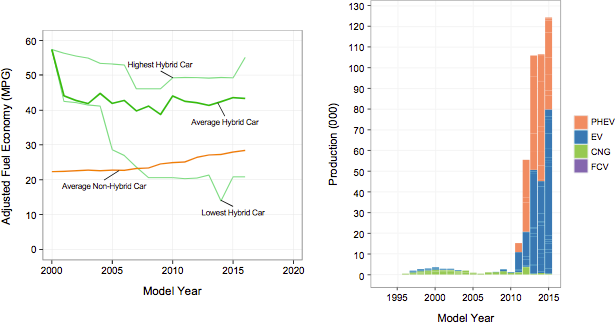
\includegraphics[width=\textwidth]{figures/review/hybrid.png}
  \caption{Comparison fuel economy between non hybrid and hybrid cars and hybrid cars production \label{fig:hybrids} }
\end{figure}


While the average fuel economy of hybrid cars remains higher than the average fuel economy  of non-hybrid cars, the difference appears to be narrowing. Average hybrid car fuel economy  has been relatively stable since MY 2001, while the fuel economy of the average non-hybrid car has increased more than 27\%. Since MY 2004, the difference in fuel economy between the average hybrid midsize car and the average non-hybrid midsize gasoline car has narrowed from about 25 mpg to about 14 mpg. The primary reason for this trend is continued improvements to the internal combustion engine. Additionally, many technologies introduced or emphasized in early hybrids, such as improved aerodynamics, low rolling resistance tires, and increased use of lightweight materials, have also become more common on non-hybrid vehicles~\cite{EPA2016}.

\subsection{The importance of waste heat recovery}

In the previous sections a brief review of how some of the key technical improvements have modified engine design, performances and fuel consumption have been provided.

One of the main causes of the relatively low efficiency of even modern ICEs is that a significant amount of energy produced by fuel combustion is wasted in form of heat, then not used to produce useful power. In internal combustion engines, only a small part of the fuel energy flow is transformed into power available at the crankshaft. For the best points of operation, diesel engines have a maximum efficiency approaching 45\% while gasoline engines have efficiencies of about 35\%. For both engines, the most part of the fuel energy flow is therefore lost as coolant heat flow and exhaust gases heat flow. In everyday operating conditions, cars have average engine efficiencies on driving cycles well below their top values, with the heat flow lost in the exhaust gases and the engine coolant increasing accordingly. In many driving conditions, the waste heat flow represents an important part of the fuel energy flow. The energy flow potentially available to be converted to usable power in the exhaust gases and the coolant is therefore quite significant~\cite{Boretti2012}. Considering the large number of vehicles in the world, such waste energy makes great impact to our environment globally.

\begin{figure}[ht]
  \centering
  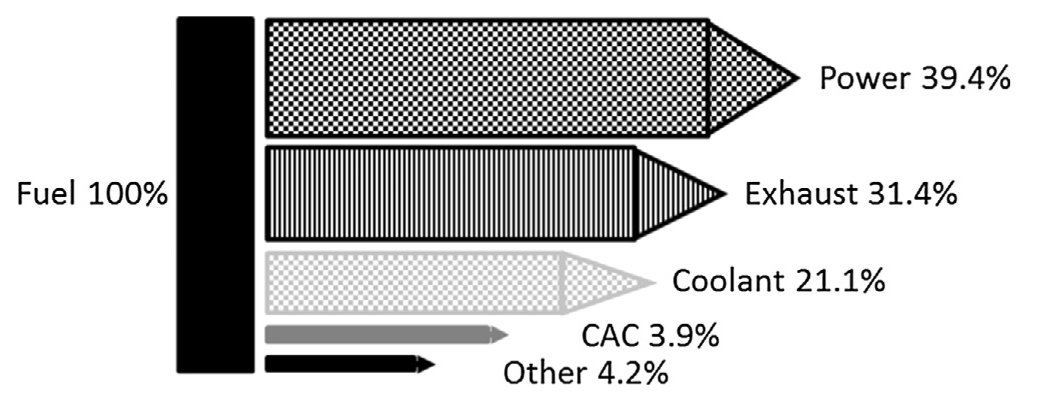
\includegraphics[width=0.6\textwidth]{figures/review/sankey.png}
  \caption{Typical energy balance of a Euro 6 diesel engine\label{fig:sankey_energy} }
\end{figure}
~

It has been estimated that the thermal efficiency of a modern IC engine is limited to 20 - 40\% while 33\% of the fuel energy from a typical medium-size passenger vehicle is carried away by exhaust gases and 29\% is carried away by engine cooling water in urban traffic conditions. Depending on engine type and operating conditions, the IC exhaust gas temperature usually varies from 500 to \SI{900}{\celsius} and engine cooling water temperature is around \SI{100}{\celsius}. It is reported that for a typical light duty 4 cylinder spark ignition engine, the waste energy carried by the exhaust gas ranges from 4.6 to 120 kW and cooling water heat ranges from 9 to 48 kW \cite{ElChammas2005}, which makes the exhaust gas and engine cooling heat very attractive for energy recovery. It's possible to harvest part of this waste energy from vehicles and produce regenerated mechanical or electrical power.

According to \cite{Conklin2010}, experimental data coming from a series of tests on a turbo-charged 2007 Saab vehicle shows engine-out exhaust temperature from 400 to \SI{600}{\celsius}. The exhaust temperature range of naturally aspirated gasoline engine is higher, typically from 450 to \SI{800}{\celsius}. The same research performed a FTP-75 test cycle with the aforementioned vehicle, and measured that the total fuel energy consumed during the course of the driving cycle is approximately 58.5 MJ, or about 1.7 L of unleaded gasoline fuel. The percentage of fuel energy converted to useful work for this driving cycle (i.e. the vehicle thermal efficiency) is 10.4\%. A much larger portion of fuel energy, 27.7\%, exits the vehicle in the form of thermal energy in the exhaust, while the remaining 61.9\% of the energy balance consists of energy losses to friction, coolant, and other. Only a portion of the energy in the exhaust is available for recovery due to process irreversibilities, ambient conditions, or other.

% BEGIN RECEIVE ORGTBL first_second_law
\begin{table}
  \begin{center}
    \begin{tabular}{lrr}
      & 1st law & 2nd law \\
      \hline
      Brake work & 10.4\% & 9.7\% \\
      Exhaust & 27.7\% & 8.4\% \\
      Irreversibilities, Friction, Coolant, and other & 61.9\% & 81.9\% \\
    \end{tabular}
    % % END RECEIVE ORGTBL first_second_law
    % \begin{comment}
    %   #+ORGTBL: SEND first_second_law orgtbl-to-latex
    %   |                                                 | 1st law | 2nd law |
    %   |-------------------------------------------------+---------+---------|
    %   | Brake work                                      |   10.4% |    9.7% |
    %   | Exhaust                                         |   27.7% |    8.4% |
    %   | Irreversibilities, Friction, Coolant, and other |   61.9% |   81.9% |
    % \end{comment}
    \caption{1\textsuperscript{st} and 2\textsuperscript{nd} law of thermodynamics fuel energy and exergy distributions}
    \label{table:1st_2nd_law}
  \end{center}
\end{table}

In Table~\ref{table:1st_2nd_law} are reported the energy and exergy distributions with respect of the fuel entering the engine. It's possible to notice how, according to the 2\textsuperscript{nd} law of thermodynamics, the exhaust exergy is nearly as high as the amount of brake work. Thus, there is an abundant amount of available energy present in the exhaust of modern gasoline vehicles that can be used to improve overall system efficiency if an effective means of energy recovery can be employed. In another research \cite{Dolz2012}  the value of exhaust gases mentioned to be 18.6\% of total combustion energy. It is also found that by installing heat exchanger to recover exhaust energy of the engine could be saved up to 34\% of fuel saving \cite{Wang2013}.

Many studies highlighted the validity of the idea of recovering this waste heat to produce additional power, and the research and actual production efforts showed promising results. In Table~\ref{Table:ORC_research_list} are listed some of the most relevant research and production vehicles equipped with a waste heat recovery system, among with the achieved increase in thermal and mechanical efficiency.

\begin{table}[]
  \centering
  \resizebox{\textwidth}{!}{
    \begin{tabular}{lllllll}
      \hline
      Reference                        & Year & Vehicle       & Heat Source                 & Research method & $\Delta\eta_{th}$ & $\Delta\eta_{mec}$ \\ \hline
      \cite{Oomori1993b}               & 1993 & Passenger car & Coolant                     & Experiment      & /                 & 3\%                \\
      \cite{ElChammas2005}             & 2005 & HEV           & Exhaust                     & Numerical       & 1.3-5\%           & /                  \\
      \cite{Arias2006}                 & 2006 & Prius         & Exhaust + engine block      & Numerical       & 5.50\%            & /                  \\
      \cite{Endo2007, Kadota2008}      & 2007 & HEV           & Exhaust                     & Experiment      & 3.80\%            & /                  \\
      \cite{Freymann2008}              & 2008 & 3 series      & Exhaust + Coolant           & Experiment      & 5.70\%            & /                  \\
      \cite{Duparchy2009}              & 2009 & HEV-Prius     & Exhaust + Coolant           & Numerical       & /                 & 9\%                \\
      \cite{He2011, ZHANG2011}         & 2011 & Toyota 8A-FE  & Exhaust, Lubricant, Coolant & Experiment      & 12-17.3\%         & /                  \\
      \cite{Freymann2012, Horsta}      & 2012 & 5 series      & Exhaust                     & Experiment      & /                 & 6\%                \\
      \cite{Boretti2012, Boretti2012a} & 2012 & 1.8L engine   & Exhaust + Coolant           & Numerical       & 1.7-5.1\%         & /                  \\
      \cite{Wang2016a}                 & 2012 & BL18T engine  & Exhaust + Coolant           & Numerical       & 3-6\%             & /                  \\
      \cite{Domingues2012}             & 2013 & 2.8L VR6      & Exhaust                     & Experiment      & /                 & 2.64-6.96\%        \\ \hline
    \end{tabular}}
  \caption{Research results on waste heat recovery benefits}
  \label{Table:ORC_research_list}
\end{table}

\section{Objectives and structure of the thesis}

The main objective of the thesis is to compare three different technologies that aim at recovering waste heat produced by the internal combustion engine. In particular, two different \emph{Organic Rankine} bottoming \emph{Cycles} (ORC) paired with an Otto-cycle engine, and a \emph{Split-Cycle Engine} with \emph{isothermal compression} and \emph{integrated waste heat recovery}.

The comparison will be performed via MATLAB/Simulink simulations. A backward-looking model will take as input the velocity profile of a driving cycle for which experimental data is available, then the torque and angular speed at the engine will be calculated through a simulated transmission. Furthermore, engine maps will be extracted from experimental data along with characteristics and performances of the heat exchangers, making possible the calculation of flow rate, temperature and heat flux for both the exhaust gases and the coolant. Once the waste heat data will be available, the bottoming cycle model will be introduced. Starting from the output of the powertrain model, the recovered energy and produced power will be calculated.

\emph{ADD METHODOLOGIES MODEL SPLIT-CYCLE}

\emph{TO BE CONTINUED WITH STRUCTURE}


%%% Local Variables:
%%% mode: latex
%%% TeX-engine: xetex
%%% TeX-master: "thesis"
%%% End:
%%% \end{document}


%%%%%%%%%%%%%%%%
% Chapter 2
%%%%%%%%%%%%%%%%

\chapter{Review of the state of the art}

\section{Introduction to bottoming recuperative cycles}

A bottoming cycle is a waste-heat recovery thermodynamic cycle that recaptures the unused energy and uses it to produce steam to drive a steam turbine generator to produce additional energy. In Figure~\ref{fig:bottoming} is shown a general configuration for a bottoming cycle. In the passenger case car, the thermal process upstream the cycle is the internal combustion engine itself.

\begin{figure}[ht]
  \centering
  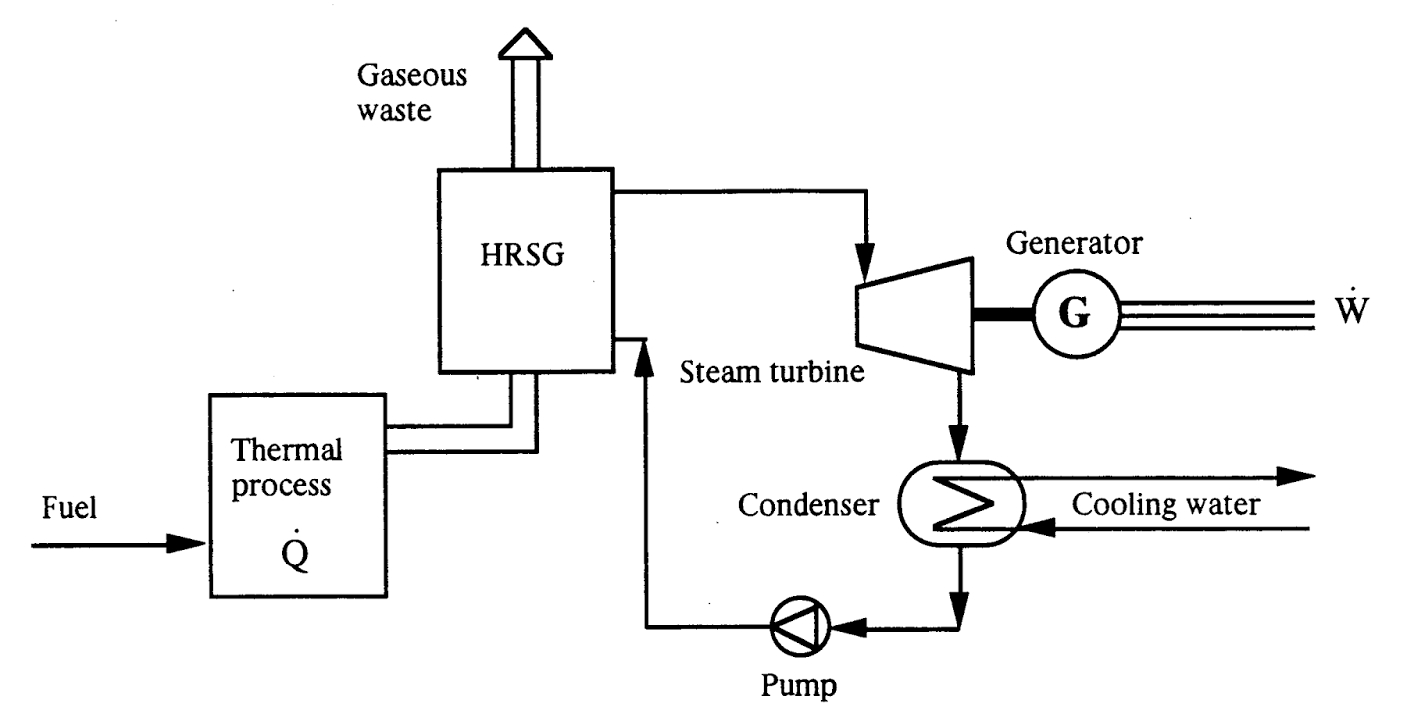
\includegraphics[width=0.7\textwidth]{figures/review/bottoming.jpg}
  \caption{Bottoming cycle \label{fig:bottoming} }
\end{figure}
~

A bottoming cycle is a powerful mean to recover the waste heat produced by an automotive internal combustion engine, and the additional power produced can be employed in different ways. It is possible to produce additional mechanical work, increasing the torque at the shaft, or produce electrical work that can be employed in different ways. Usually the selected recovery strategy is to use the recuperative cycle to produce mechanical power: this implementation is simpler and effective, but fails to achieve the maximum potential with respect to the operative conditions of the additional cycle. In this configuration the angular speed of the turbine is the same as the one of the shaft, but this speed can be different from the one of maximum efficiency of the turbo-machine.

The configuration that converts the additional power in electrical power can solve this issue. Being the system no more coupled with the shaft of the internal combustion engine but with an electric generator, the rotational speed of the turbine can be varied at will in order to achieve the most efficient operative point. The electricity produced can be stored in batteries is they are available (i.e. Hybrid or Plug-in vehicle), or used to power up auxiliaries and reduce the alternator load on the engine.

In the following sections a brief overview of the most common thermodynamic cycles that can be used as a recuperative bottoming cycle will be provided.

\subsection{Steam Rankine cycle}

The steam Rankine cycle is one of the most famous and used thermodynamic cycles for producing power. In this cycle the heat is provided externally to a closed loop, in which water flows as a working fluid. The efficiency of the Rankine cycle can be calculated as:

\begin{equation} \label{eq:eta_rankine}
  \eta_t = \frac{\dot{W}_{thermal}-\dot{W}}{\dot{Q}_{in}} \approx \frac{\dot{W}_{turb}}{\dot{Q}_{in}}
\end{equation}

This type of cycle is commonly used in thermal power generation plants. The efficiency of the Rankine cycle is limited by the high heat of vaporization of the working fluid. Also, unless the pressure and temperature reach super critical levels in the steam boiler, the temperature range the cycle can operate over is quite small: steam turbine entry temperatures are typically around \SI{565}{\celsius} and steam condenser temperatures are around \SI{30}{\celsius}.

\begin{figure}[ht]
  \centering
  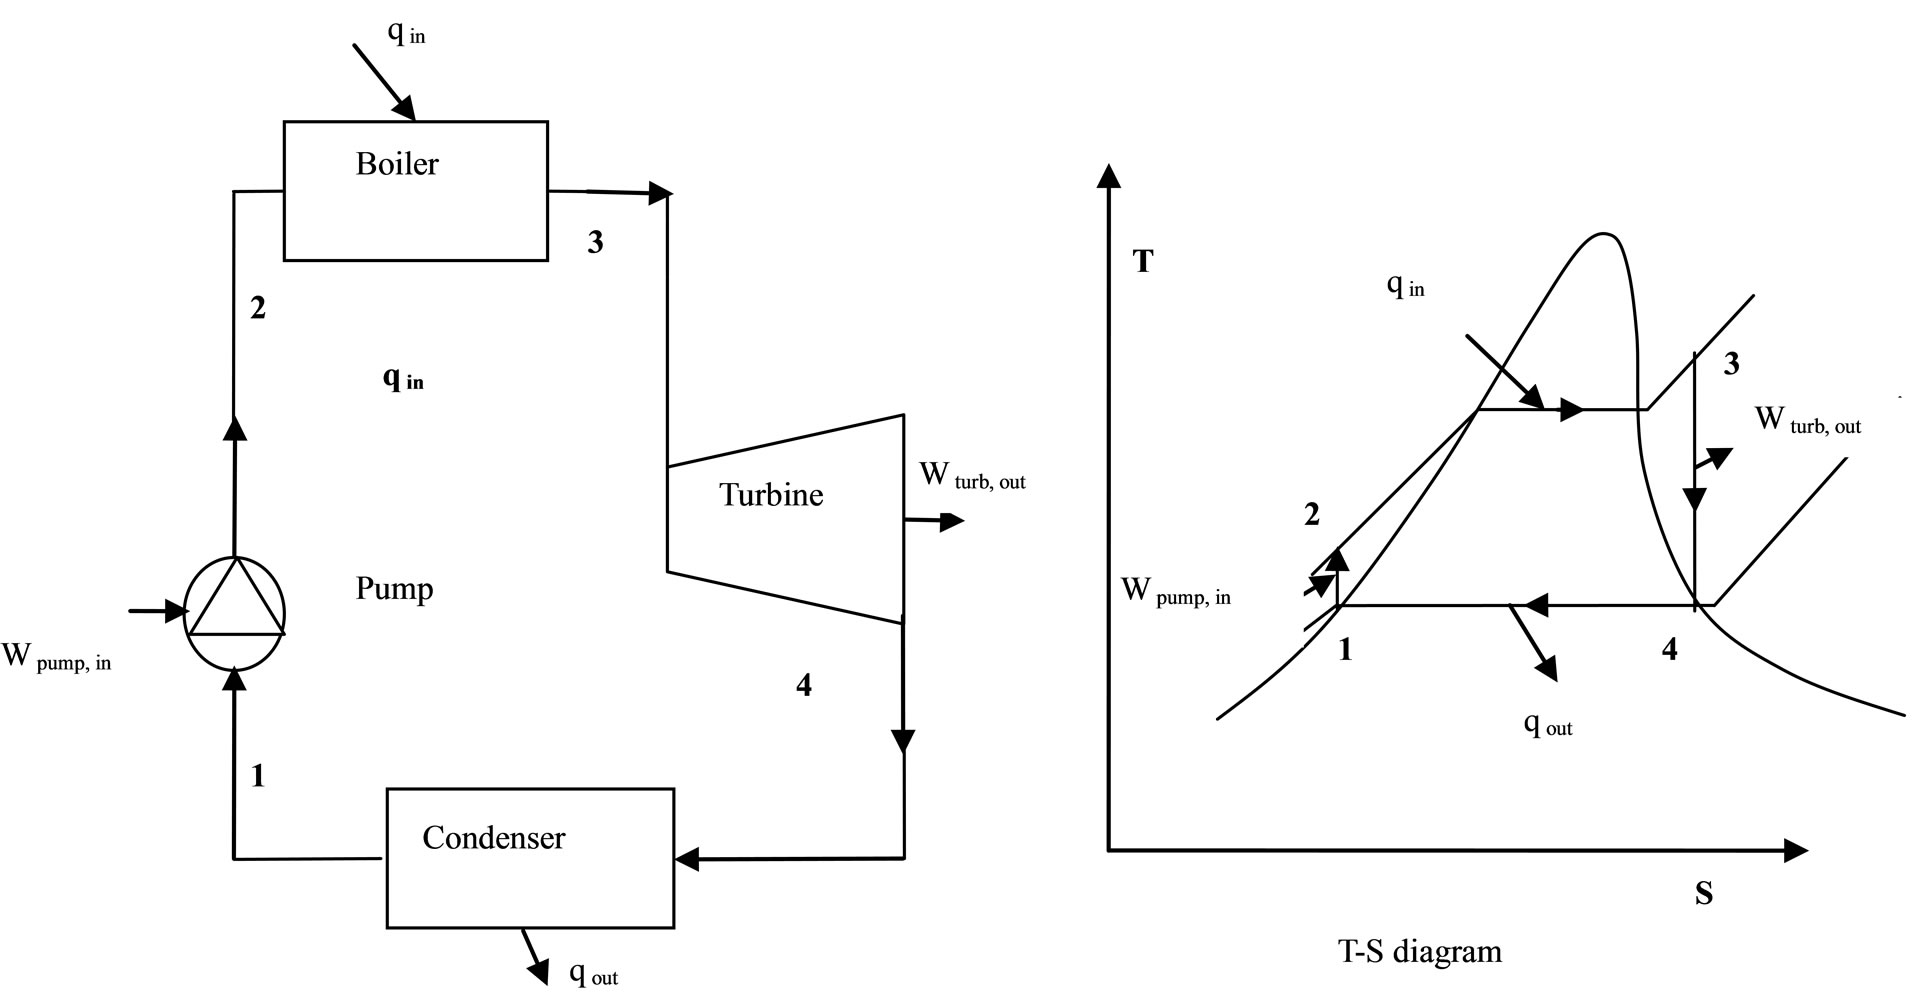
\includegraphics[width=\textwidth]{figures/review/rankine_steam.jpg}
  \caption{Steam Rankine cycle T-s diagram and physical layout\label{fig:rankine_steam} }
\end{figure}

The process is composed by four consecutive processes, as shown in Figure~\ref{fig:rankine_steam}:

\begin{itemize}
\item \textbf{Process 1-2:} the working fluid is pumped from low to high pressure. Since the fluid is in liquid form, the work required for pumping is small.
\item \textbf{Process 2-3:} the liquid at high pressure is heated at almost constant pressure by an external source until it becomes dry saturated vapor.
\item \textbf{Process 3-4:} the dry saturated vapor is expanded through a turbine, hence generating power. The working fluid experience a decrease of pressure and temperature, with possible partial condensation.
\item \textbf{Process 4-1:} the wet vapor enters the condenser and returns to saturated liquid conditions.
\end{itemize}



\subsection{Organic Rankine cycle}

The Organic Rankine Cycle (ORC) is a particular use case of a Rankine thermodynamic cycle. It's named for its use of an organic, high molecular mass fluid with a liquid-vapor phase change, or boiling point, occurring at a lower temperature than the water-steam phase change. The fluid allows Rankine cycle heat recovery from lower temperature sources such as coolant from internal combustion engines. The low-grade waste heat is converted into useful work, that can itself be converted into mechanical or electrical power. In Figure~\ref{fig:orc_diagram}, the T-s diagram and the plant layout for a generic Organic Rankine Cycle are shown. The formulation of the efficiency is the same as the Steam Rankine Cycle, shown in Equation~\ref{eq:eta_rankine}.

\begin{figure}[ht]
  \centering
  \includegraphics[width=0.8\textwidth]{figures/review/orc.jpg}
  \caption{T-s diagram and plant layout for a generic Organic Rankine Cycle\label{fig:orc_diagram} }
\end{figure}

The system itself is made of four components: evaporator, expander, condenser and pump. Usually a recuperator is also used, to increase the efficiency and hence the production of useful power. The waste heat is used in the evaporator to vaporize the working fluid and convert the heat in mechanical work in the expander.

The selection of the working fluid is of key importance in low temperature Rankine Cycles. Because of the low temperature, heat transfer inefficiencies have a major importance. In order to recover low-grade heat, the fluid generally has a lower boiling temperature than water, then refrigerants and hydrocarbons are two commonly used components. Water is a preferable working fluid for high exhaust gas temperatures ranging from \SI{500}{\celsius} to \SI{800}{\celsius}, while refrigerants are better suited fro lower temperatures, as in the gas of the exhaust gases. Water also has the disadvantage that requires superheating to avoid turbine blade erosion, but the high degree of superheating makes it less practical for automotive application due to the variation of exhaust temperature at different load conditions. In figure~\ref{fig:orc_working_fluids} are reported the different T-s diagram related to different Rankine cycle working fluids.

\begin{figure}[ht]
  \centering
  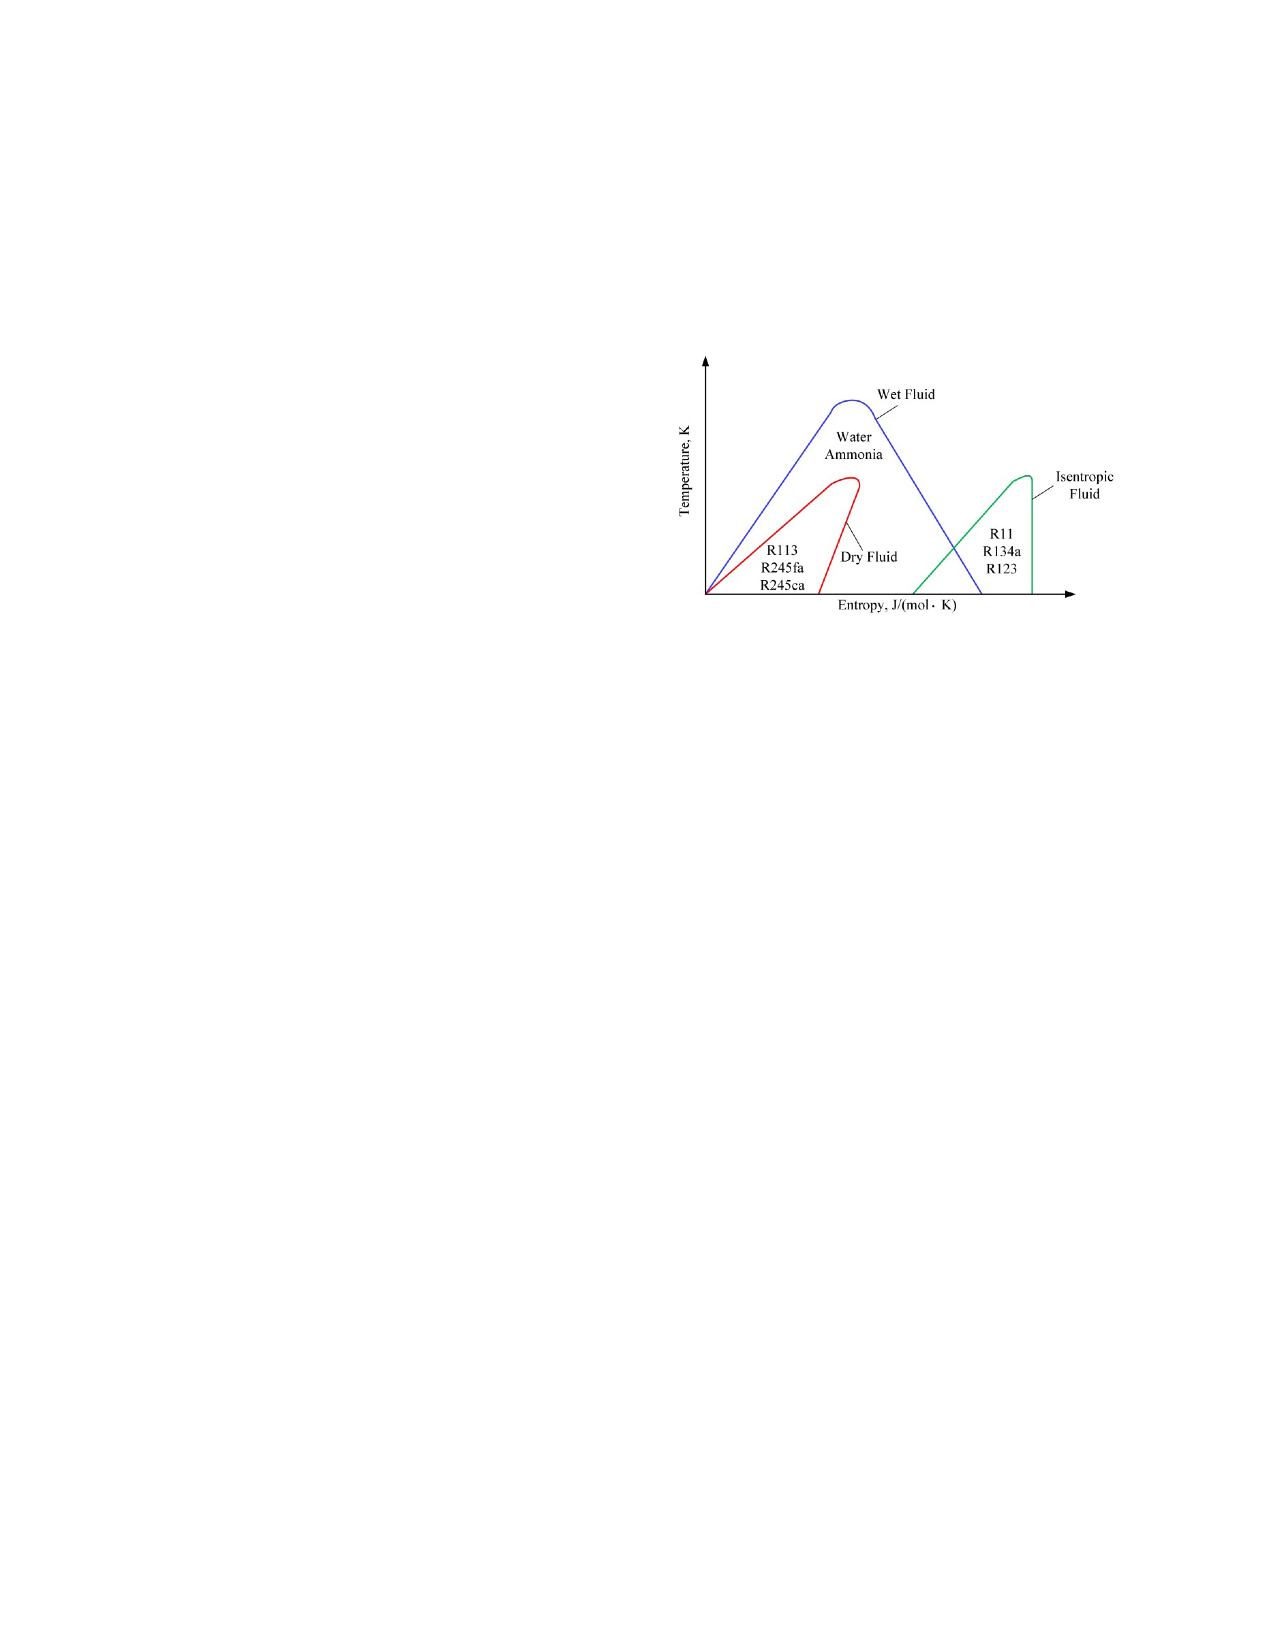
\includegraphics[width=0.7\textwidth]{figures/review/orc_working_fluids.pdf}
  \caption{Comparison of different Rankine Cycle working fluid characteristics\label{fig:orc_working_fluids} }
\end{figure}

In current years, an increasing environmental awareness has provoked the shifting from traditional refrigerants (i.e. R134a, R236fa, R245fa) to new refrigerants, characterized by lower harm potential to passengers in case of leakage or crashes, and a lower flammability level (i.e. R1233zd, R1234yf).

When considering an ORC coupled with an internal combustion engine, different possible configurations must be considered. The most common and simple structure utilizes the exhaust gas as the only heat source to evaporate the working fluid. The second structure adds another heat exchanger (recuperator) before the evaporator, using the steam from the expander to preheat the working fluid. A third structure uses waste heat from engine coolant to preheat the working fluid. The regenerative preheating of structure 2 requires a very complex liquid-gas heat exchanger with high exchange surfaces, while the preheater in structure 3 only requires a simple liquid-liquid heat exchanger. There have been contradicting conclusions about the effect of preheating using engine coolant on the RC system efficiency. Based on Vaja and Gambarotta's work \cite{Vaja2010}, the RC system with a preheater allows a net increase in power output, compared to structure 1, of 10\% to 35\%, depending on which working fluid is chosen. Alberto Boretti \cite{Boretti2012} also showed a 8.2\% fuel economy improvement using engine coolant to preheat the RC cycle, compared to a 6.4\% improvement when only exhaust gas is used to boil the working fluid. Arias et al. \cite{Arias2006} also compared the combined exhaust and engine coolant heat recovery system with the exhaust only structure. It was found that the additional power recovered from the engine coolant system was 20 W out of a total 2140 W, which is around 1\% improvement.

\begin{figure}[ht]
  \centering
  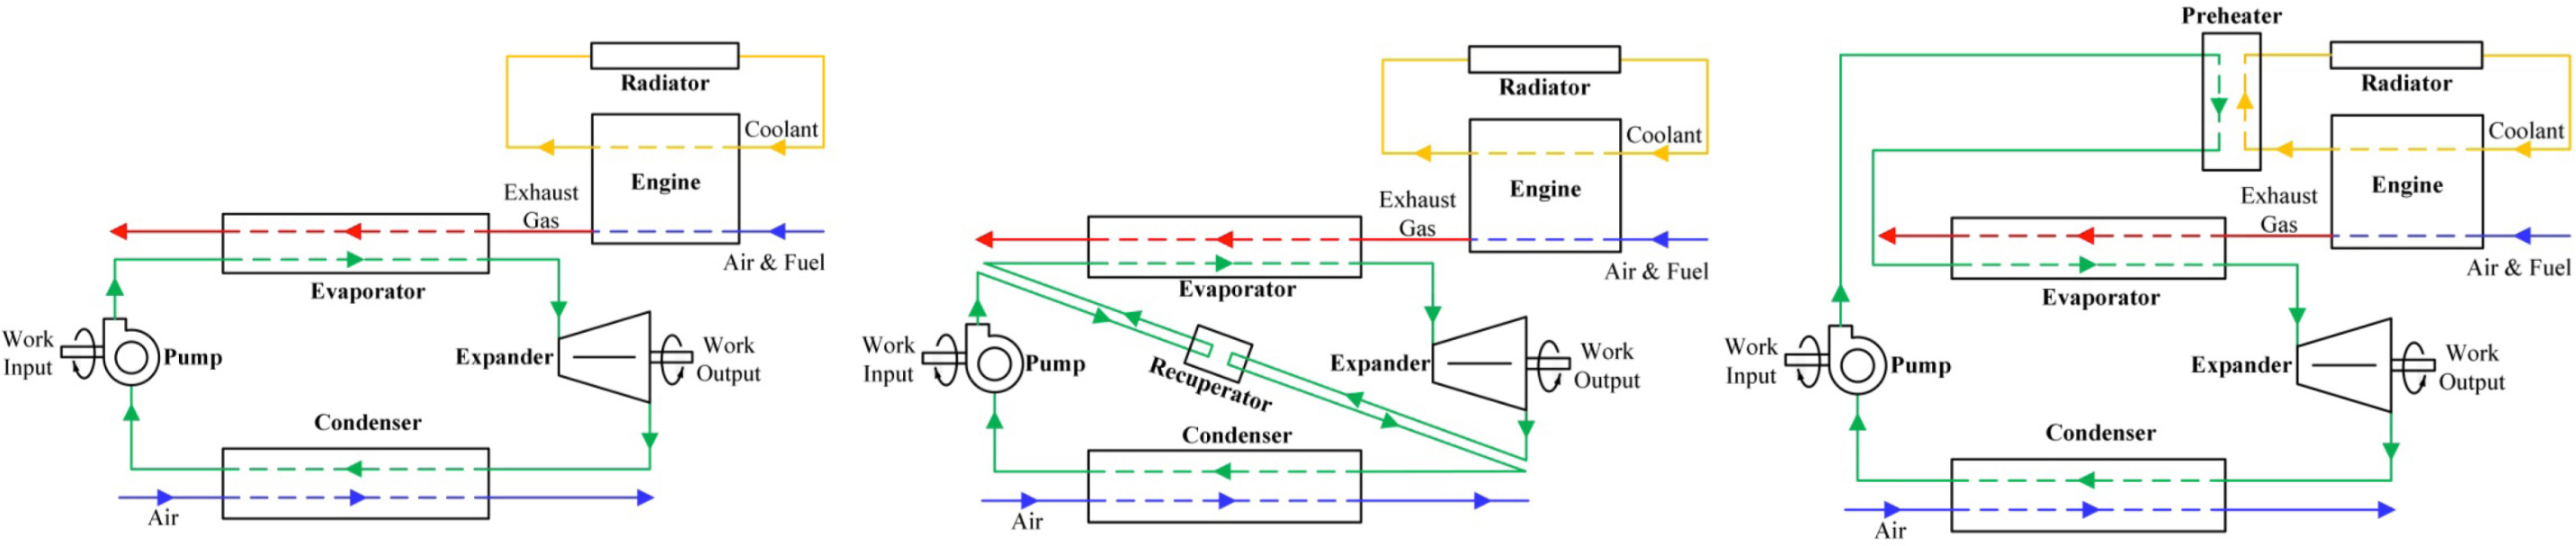
\includegraphics[width=\textwidth]{figures/review/orc_layouts.jpg}
  \caption{Different ORC layouts: structure 1, 2 and 3\label{fig:orc_layouts} }
\end{figure}

When selecting the different configurations, different factors have to be take into consideration as the maximization of the recovered energy is not the only objective to pursue. System complexity, component volume and weight, and the resulted extra cost added to the vehicles and the payback period are also big concerns.

\subsection{Brayton cycle}

The Brayton cycle is a thermodynamic cycle that uses a gas as a working fluid. The generalized plant configuration and the p-V and T-s diagrams are showed in Figure~\ref{fig:brayton_cycle}.

The cycle is composed by:

\begin{itemize}
\item \textbf{Process 1-2:} adiabatic compression, operated in a turbo-machine (compressor)
\item \textbf{Process 2-3:} isobaric heat addition, operated in the combustor
\item \textbf{Process 3-4:} adiabatic expansion, operated in a turbo-machine (turbine)
\item \textbf{Process 4-1:} isobaric heat rejection, operated in a radiator in the case of a closed cycle
\end{itemize}

\begin{figure}[ht]
  \centering
  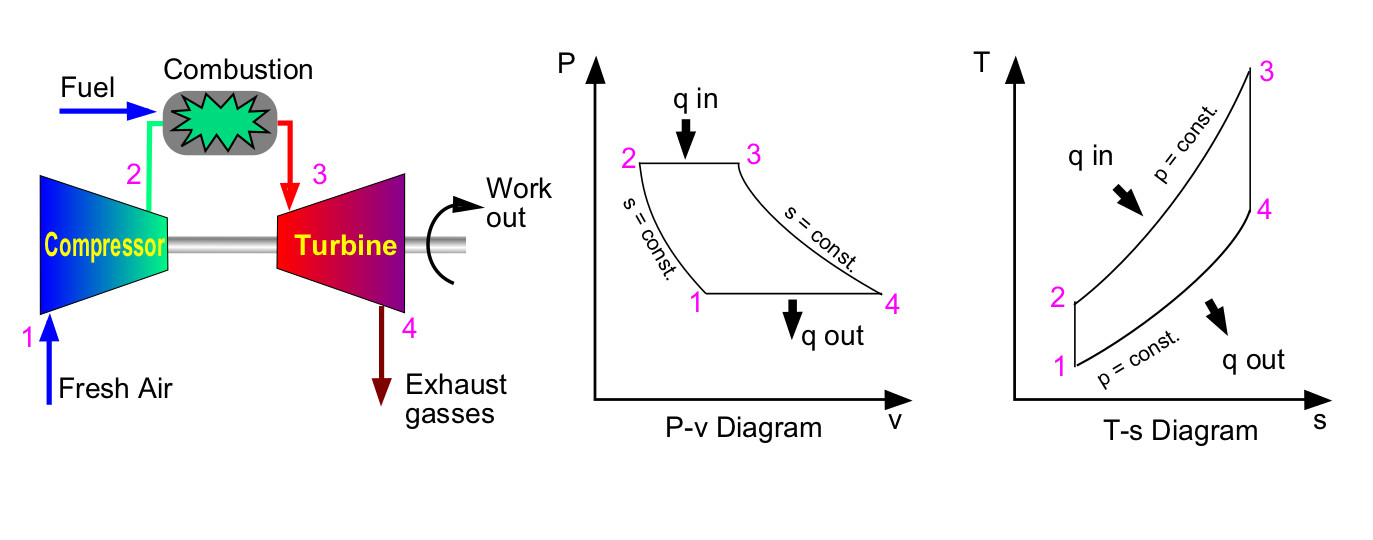
\includegraphics[width=\textwidth]{figures/review/brayton_cycle.jpg}
  \caption{Diagrams and plant layout of an idealized Brayton cycle\label{fig:brayton_cycle} }
\end{figure}


The efficiency of the cycle can be calculated as:

\begin{equation}
  \eta_{t}=1-\frac{1}{\beta^{k-1}}
\end{equation}

The regular Brayton thermodynamic cycle proved itself not to be suited for a bottoming cycle type of application. Of particular importance for waste heat recovery applications is the \emph{Super-critical CO\textsubscript{2}} (sCO2) Brayton cycle. Researchers claim \cite{Kimzey2012} that an sCO2 power cycle could potentially exhibit a higher thermal efficiency than steam cycles when operating between the same maximum and minimum cycle temperatures. In addition, the high energy density of sCO2 suggests that the size requirements for the turbomachinery used in an sCO2 power cycle could potentially be much lower than those used in steam cycle generation, which may result in lower capital costs. To date, most research in the field has been dedicated to the use of sCO2 as the primary power cycle in nuclear applications, but relatively little research has been aimed toward developing an sCO2 cycle that is well-suited to bottoming cycle applications.

\subsection{Selection of the bottoming cycle}

After having introduced the three most common thermodynamic cycles that can be employed as bottoming cycle, it's necessary to understand the up and downsides of the three in order to select the better one for the use case considered in this thesis.

The choice between the two different Rankine Cycles is basically reduces to the selection of the most appropriate working fluid. The choice of the working fluid to be used in the cycle depends on a number of factors, e.g thermodynamic efficiency, environmental protection, safety, process-related and economic issues.

The steam Rankine cycle is the most reliable and simple configuration considered, it has a high efficiency due to the very small work required for the pump. Water is widely available, cheap and does not present any issue in form of toxicity or environmental harm potential. The biggest downside of the selection of water is the huge latent heat of vaporization. According to Arias at al. \cite{Arias2006}, water is not suited to recover heat when used as a working fluid because of the mismatch between the low temperature of engine coolant and high boiling temperature of water. Water has been used in the fist generation of BMW's Rankine system \cite{Freymann2008}, the \emph{Turbosteamer}, to harvest energy from exhaust gases, while ethanol was used in a separate loop for engine coolant waste heat recovery. In the second generation Turbosteamer \cite{Freymann2012}, water is only been heated by the exhaust gases. This is because water works best when used for high exhaust gas temperature, from \SI{500}{\celsius} to \SI{800}{\celsius}. Water required also superheating to avoid turbine blade erosion, if turbine is selected as expander, but the high degree of superheating makes it less practical for the automotive application due to the variation of exhaust temperature at different load conditions. Besides, its high freezing point (\SI{0}{\celsius}) cannot meet the standard automotive working temperature range (\SI{-40}{\celsius} to \SI{85}{\celsius}).

Organic Rankine Cycle shows a much better potential for waste heat recovery in automotive applications. The low boiling point of the organic fluid allows to recover efficiently low-grade waste heat. The dry/isentropic refrigerants are widely used in small-scale RC applications because of their good heat transfer properties, excellent thermal stability and low viscosity. They are generally non-flammable, which is a big advantage for automotive application and compatible with most materials. Under typical low temperature ambient conditions they do not freeze, which is a major concern with water. Chammas and Clodic \cite{ElChammas2005} compared different organic fluids with water for RC application to hybrid vehicles, arguing that using water to recover automotive waste heat could lead to a complex system requiring large size equipment and high investment cost, which makes the study on organic working fluid necessary. Domingues et al. \cite{Domingues2012} compared R123 and R245fa with water as working fluid for vehicle RC waste heat recovery potential from exhaust gas. The study revealed the advantage of using water as working fluid to recover waste heat from exhaust gas of vehicles equipped with spark-ignition engine. However, it was also found that the heat exchanger effectiveness for R123 and R245fa is higher than that for water. Consequently, when the exhaust temperature is relatively low, organic fluids can be considered appropriate for vehicle RC application. Extensive work has also been poured in ORC + internal combustion engines combinations, leading to interesting fuel saving values.

The usage of organic fluids, such as refrigerants (i.e. R134a, R245fa, etc.) carries a few shortcomings. First, the intrisic property of dry/isentropic fluids reduce the area of net work in the T-s diagram, which means less power output compared to wet fluid, e.g. water. Second, to reduce the cooling load of the condenser, a recuperator is usually necessary to cool the superheated vapor to saturated state, increasing the system complexity and cost. Moreover, most organic fluids have relatively low thermal instability temperatures compared to water, therefore at high temperature and pressure the system might suffer chemical decomposition and deterioration. In addition, the current generation of refrigerants has a high global warming potential, which means that their use could be limited or banned in the near future.

The super-critical CO\textsubscript{2} Brayton cycle combines the advantages of both steam Rankine cycle and gas turbine system. In other words, the fluid is compressed in the incompressible region, and the higher turbine inlet temperature can be utilized with less material issues compared with the steam Rankine cycle. Therefore, the volumetric flow rate decreases as the fluid density is higher, resulting in 10 times smaller turbomachinery compared with the turbomachinery of a steam Rankine cycle \cite{Ahn2015}. In addition, researchers claim \cite{Kimzey2012} that an sCO2 cycle could potentially exhibit a higher thermal efficiency than steam cycle, when operating between the same maximum and minimum temperatures. A modeling research performed by Kimzey \cite{Kimzey2012} highlighted that the Brayton cycles are well suited to operating with a heat flux producing power source, but are not well suited to a sensible heat source, such as topping cycle exhaust. This is because this cycle is not truly effective at recovering waste heat: most Brayton cycles are not self-sustaining at operating temperatures below \SI{480}{\celsius}, a problem that revealed itself also in solar thermal plants. 

Given the above reasons, in this thesis an Organic Rankine Cycle has been selected as bottoming cycle to be modeled and coupled with the 3.6L V6 petrol engine Simulink model.

\section{Introduction to split cycle engines}

In the following chapter, an introduction to the basic concept of the split-cycle engine, and of alternative methodologies for recover waste heat will be provided. In the last decades engine improvements through friction reduction and improvements in the combustion system has been the main drivers, but savings will become increasingly difficult and costly \cite{Stanton2013}. The aim of this section is to introduce a different design that has the potential to achieve better results than the conventional one in terms of both efficiency and power density. The aforementioned approaches, combined with waste heat recovery, are likely to yield a maximum system efficiency of 45-50\%. Further improvements to efficiencies beyond 50\% require a fundamental change to ICE cycle \cite{Dong2015}.

\subsection{Basic principles}

In a conventional Otto cycle engine, each cylinder performs four strokes per cycle: intake, compression, power, and exhaust. This means that two revolutions of the crankshaft are required for each power stroke. The split-cycle engine divides these four strokes between two paired cylinders, a concept first described by Ricardo in 1908, and further developed by Carmelo Scuderi. Scuderi developed a modified version of the split-cycle engine, and filed the first patent for the \emph{Scuderi Split Cycle} (SSC) in 2001 \cite{Scuderi2003}, followed by supporting patents. The SSC concept divides the four strokes of a conventional combustion engine cycle over two paired cylinders. The first cylinder, referred to as the compressor, provides intake and compression strokes. The second cylinder, referred to as the expander, provides power and exhaust strokes. The two cylinders are connected by a crossover port through which the high pressure gas is transferred from the compressor cylinder to the expander cylinder between the compression and power strokes. The splitting of the compression and expansion strokes into separate cylinders has the potential to greatly improve the overall cycle efficiency. In Figure~\ref{fig:split_simple} \cite{gentili2014split}  is reported the general plan layout for a simple split cycle engine. In blue is the compression cylinder, in yellow the crossover, and in red the combustion cylinder.

\begin{figure}[ht]
  \centering
  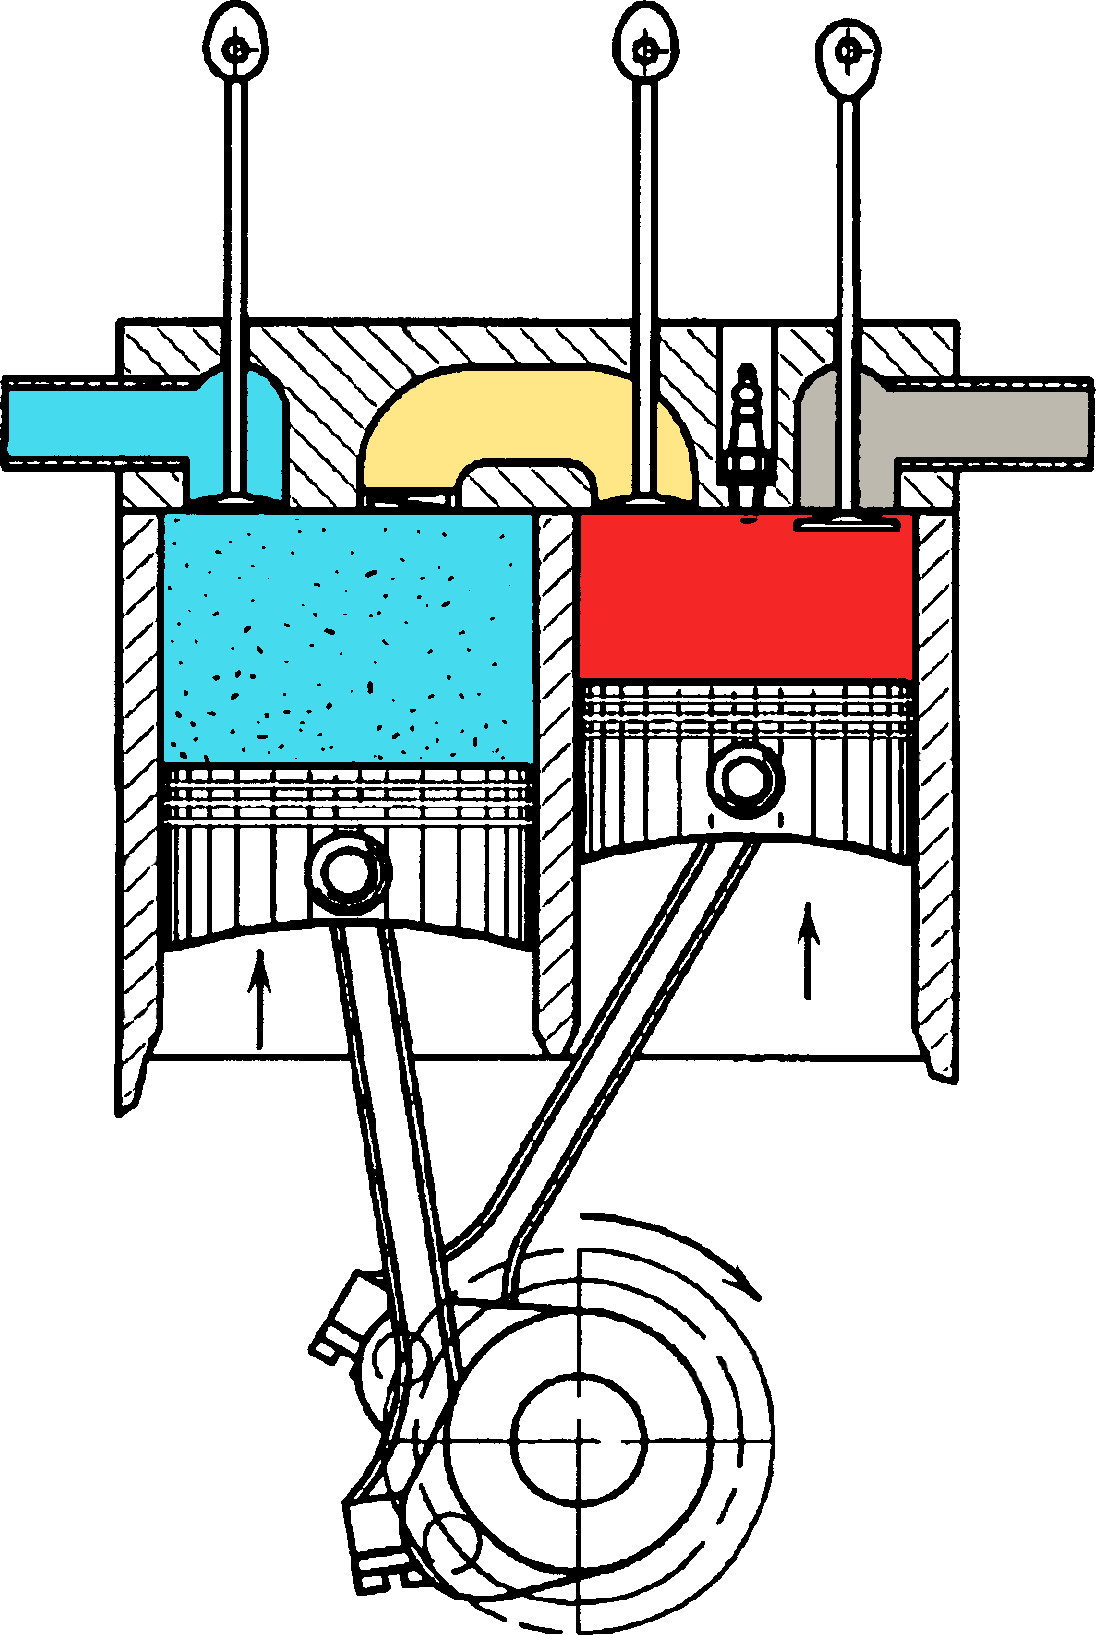
\includegraphics[width=0.5\textwidth]{figures/review/split_engine_view.png}
  \caption{Simplest plant layout for a split cycle engine\label{fig:split_simple} }
\end{figure}

A major functional benefit of the split-cycle as an internal combustion engine is the separation of compression and power strokes, which allows increased flexibility in optimizing these processes and designs. Other benefits are the ability for substantial Miller/Atkinson cycle type operation as extended expansion during the power stroke compared to compression stroke, or pressure charging the expander with the compressor, by use of differing compressor and expander displacements. Additionally, the crossover port arrangement enables charge motion, fuel and air mixing and combustion enhancement by means of the high pressure gas transfer from the crossover port to the expander. For SI applications, fuel injection can either be direct injection into the expander cylinder, or port injection into the crossover port during the gas transfer from the compressor into the expander (or both). Either method of injection results in less time for fuel chemical reactions leading to pre-ignition (or knock) than with intake port fuel injection used on conventional SI engines \cite{Phillips2011a}. The beneficial effects of such an engine configurations are also the reduction of the compression work, due to induction into a cool cylinder or direct cooling of the charge air during compression and the possibility of high pressure waste heat recovery between the compression and combustion cylinders.

Possible losses to be minimized in a split cycle engine are the flow pumping losses past the crossover valves and through the crossover ports, and energy losses due to heat transfer from the compressed air to the crossover port walls. Since the compressor cylinder has two cooler strokes, and the power cylinder has two hotter strokes, managing thermal loading is also a challenge for split cycle engines \cite{Phillips2011a}. 

Starting from the work of Coney et al. \cite{Coney2004}, the concept of isothermal compression has been applied to the split cycle engine to further improve its efficiency capabilities. Isothermal compression has the potential to reduce the after-compression temperature of the working fluid. By injecting the coolant media, such as liquid nitrogen or water, into the working fluid, the temperature of the compressed working fluid can be decreased significantly. It can be lower than the after-expansion temperature of the working fluid exiting the expansion cylinder. This allows to recover an increased amount of heat from the exhaust gases. This innovative methodology for waste heat recovery has been called \emph{intra-cycle waste heat recovery} (ICWHR) \cite{Coney2004, Dong2015, Morgan2016}. The split cycle engine structure design allows the compression and expansion processes to happen in separate chambers, and then heat recuperation is achieved through a recuperator installed between the two chambers. Due to the isothermal compression of the charge air, the temperature difference between the compression and expansion chamber is significant, allowing an efficient recuperation.

\subsection{Split-cycle engine operation}

In the following section the principles of engine operation for the split cycle will be explained, in terms of valve timing and crank angles. The timings are referred to the Scuderi version of the engine, and are based on the work of Phillips and al. \cite{Phillips2011a}.

\begin{figure}[ht]
  \centering
  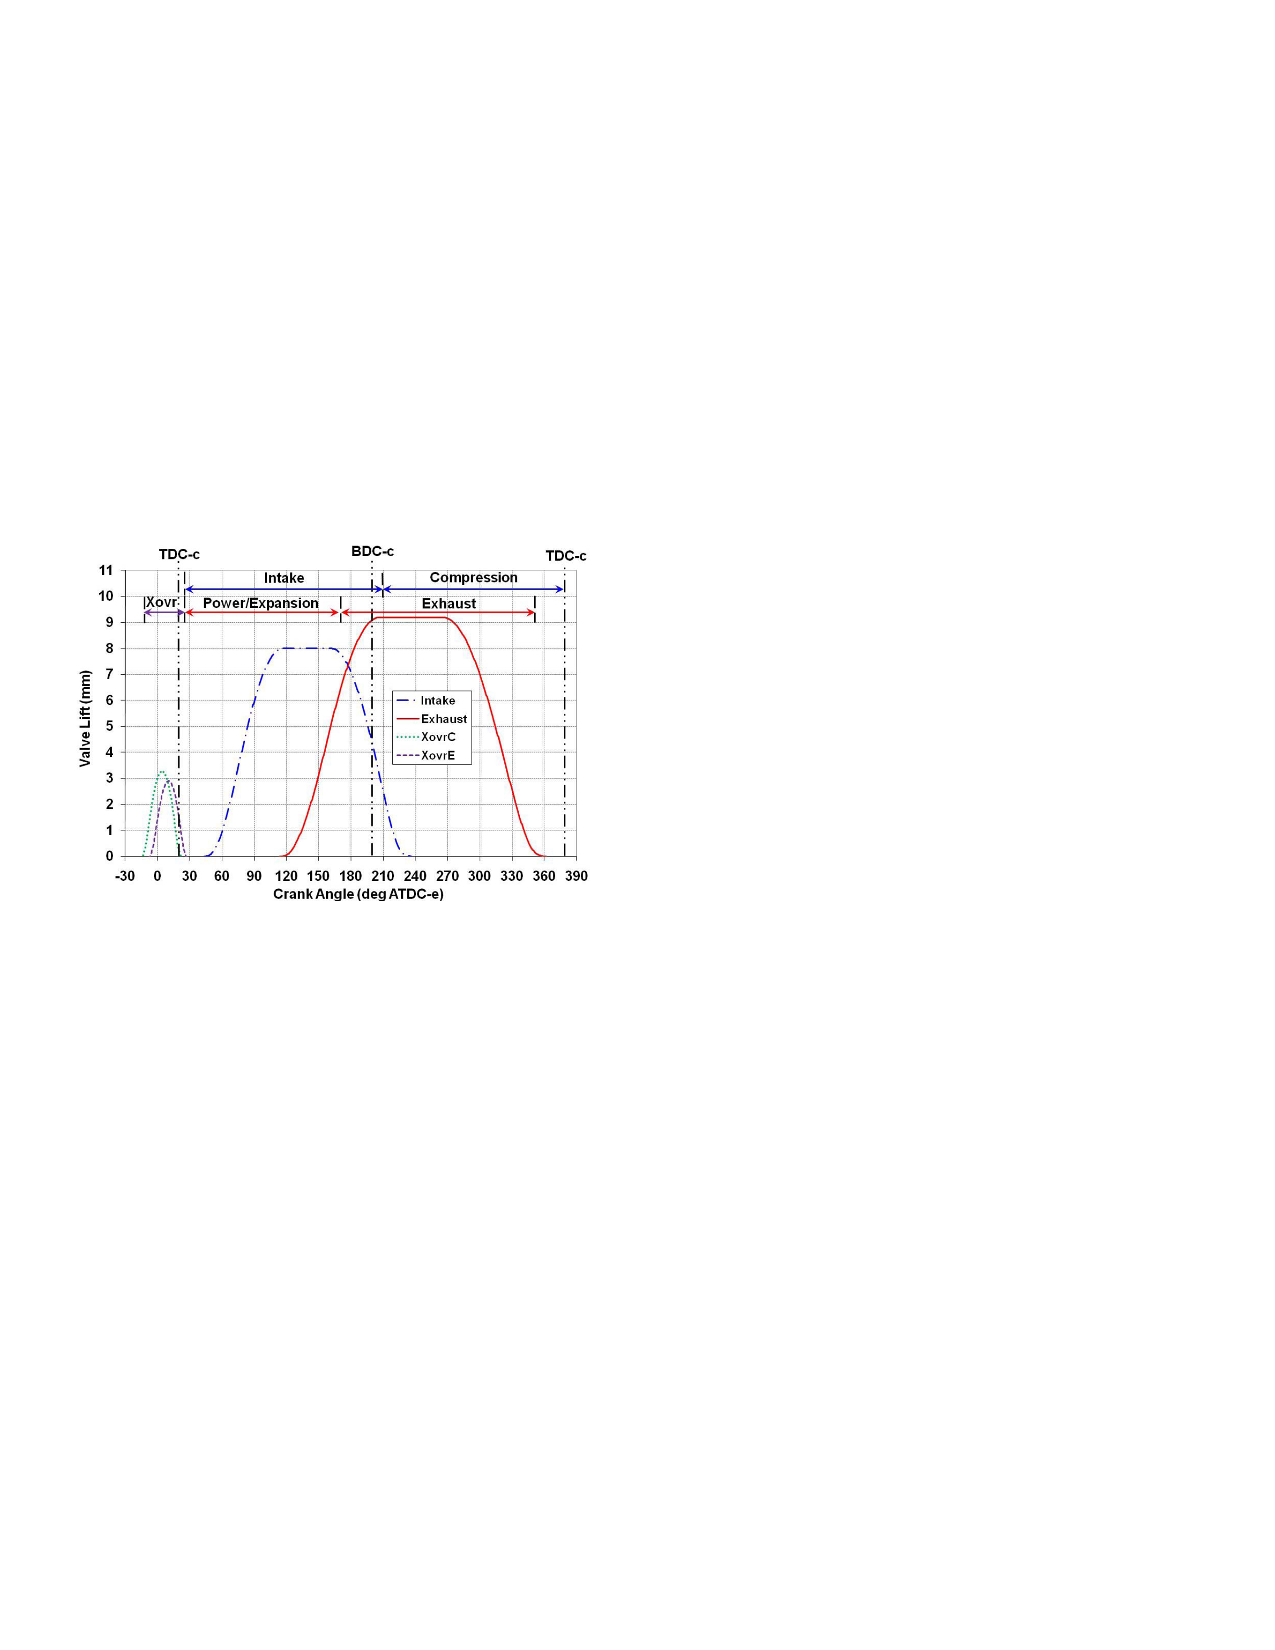
\includegraphics[width=\textwidth]{figures/introduction/split_timing.pdf}
  \caption{Valve events for SSC engine at 4000 RPM and full load conditions\label{fig:split_timing} }
\end{figure}

Figure~\ref{fig:split_timing} shows typical valve events for the engine. The compressor top dead center (TDC) is phased 20 degrees later than the expander TDC, and thus its crank angle scale is offset 20 degrees later than the expander scale shown. The Scuderi cycle begins at intake valve opening (IVO) of the compressor. For this operating point intake valve closing (IVC) is after BDC of both cylinders. Full variable valve actuation (VVA) is needed, so that the IVC varies with speed and load, and thus early IVC is used in combination with the intake throttle to control engine mass air flow. Compression takes place from IVC until TDC of the compressor cylinder, and overlaps the openings of the valves at the ends of the crossover (Xovr) ports, both at the compressor end (XovrC valves) as well as at the expander end (XovrE valves). In addition to the 4 phases of the conventional 4-stroke cycle, the SSC Xovr port provides a modulated high pressure gas transfer phase from compressor to expander cylinders between and overlapping the compression and power strokes. Prior to or slightly after XovrE valves open, fuel injection begins into the Xovr ports just ahead of the XovrE valves, and air and fuel mix enters the expander cylinder. As XovrE valves are nearly closed, spark ignition begins the power stroke. The power stroke ends when the exhaust valve opens (EVO) in the expander cylinder; the valve closes (EVC) just before TDC-e, ending the Scuderi cycle. Note that with fully variable intake and exhaust valve events, IVO, IVC, EVO and EVC timings can be varied with engine speed and load to optimize performance.

As the combustion takes place in an expanding cylinder, the peak temperatures are significantly lower than in a conventional engine leading to greatly reduced NOx formation. All gas-exchange and thermodynamic events are repeated every engine revolution such that the SSC can be viewed as a 4-stroke engine operating over two simultaneous 2-stroke cycles.
After

\subsection{Intra-cycle Waste Heat Recovery}

In this section the advantages and some implementation aspects of ICWHR will be presented and discussed. Figure~\ref{fig:ICWHR_vs_ORC}a shows the different energy fluxes that are related to an integrated waste heat recovery and to a bottoming cycle recovery.

\begin{figure}[ht]
  \centering
  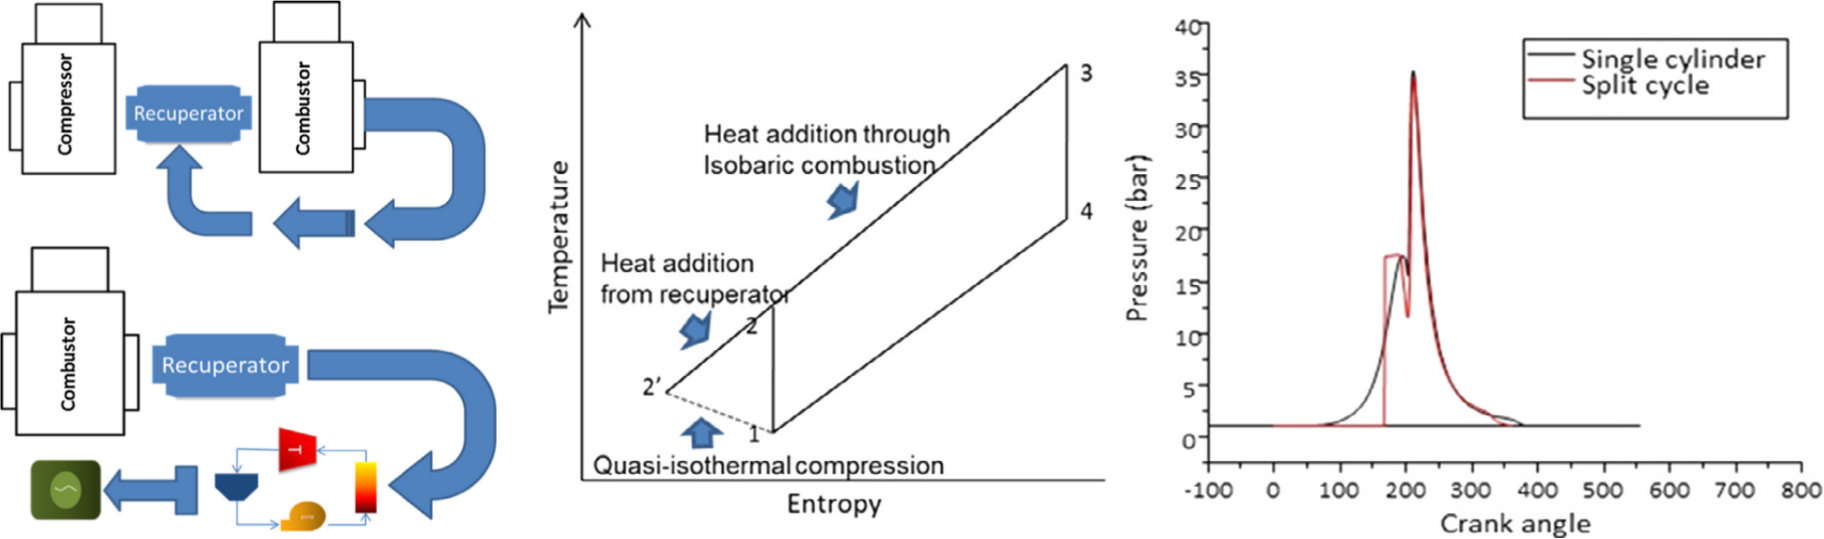
\includegraphics[width=\textwidth]{figures/review/ICWHR_vs_ORC.pdf}
  \caption{a) Comparison of the energy fluxes between an intra-cycle waste recovery and bottoming cycle type recovery, b) T-s and p-crank angle diagram for a split cycle engine with ICWHR\label{fig:ICWHR_vs_ORC} }
\end{figure}

As shown in Figure~\ref{fig:ICWHR_vs_ORC}b, the T-s diagram of the split cycle with the addition of the ICWHR is slightly different from the one showed before in Figure~\ref{fig:split_simple} due to the quasi-isothermal nature of the compression and the heat addiction coming from the recuperator.

A quasi-isothermal compression can be achieved by means of injection of water, or liquid nitrogen, during the compression phase in the first cylinder. Through the heat transfer between the intake air and the water spray droplets, the air temperature at the end of the compression stage can be decreased. The remaining liquid at the end of the compression phase can be removed using a separator.

\begin{figure}[ht]
  \centering
  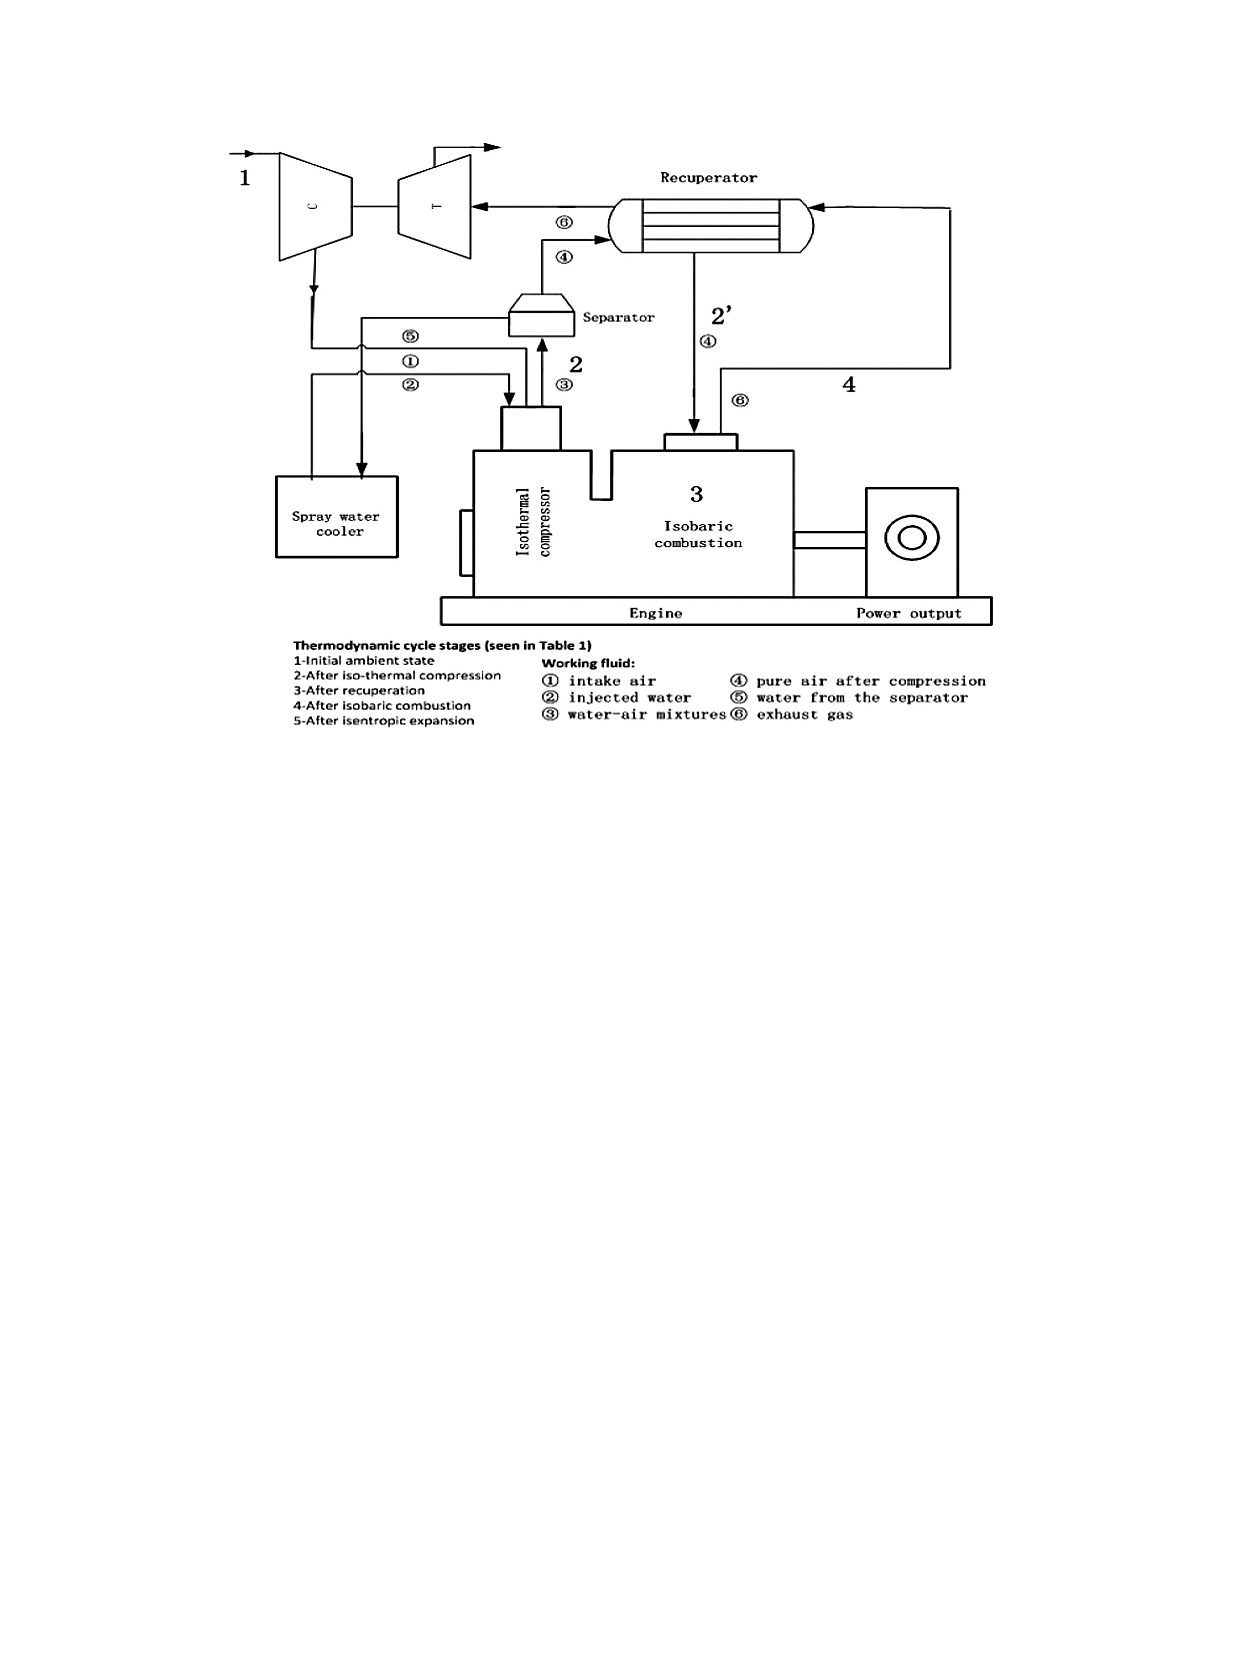
\includegraphics[width=0.8\textwidth]{figures/review/split_ICWHR_layout.pdf}
  \caption{Schematic of the engine equipped with quasi-isothermal compression and ICWHR\label{fig:split_ICWHR_layout} }
\end{figure}

In Figure~\ref{fig:split_ICWHR_layout} the layout of the engine with quasi isothermal-compression and ICWHR is shown. Ambient air (1) is pre-compressed in  turbocharger, and then sent to the reciprocating compression cylinder (2). Water is injected into the cylinder to cool down the air during compression, resulting in a quasi-isothermal compression process. After the compression stage (3), a high pressure two-phase water/air mixture leaves the isothermal compressor, and the water is recovered in a separator. The liquid water is cooled and sent back to a water tank (5). A recuperator is installed downstream the separator to heat the high-pressure air (4). Within the recuperator, the air is heated by the exhaust flow (7), and then an intra-cylinder heat recovery process is achieved. After the recuperation process (6), the fully preheated compressed air is fed to the combustion cylinders. As the combustion chamber intake valve opening time (IVO) is near to top dead centre (TDC), the diffusion of the combustion flame occurs in the expansion stroke of the cylinder. As a result, the combustion peak pressure is not increased significantly and a quasi-isobaric combustion process can be assumed. At the end of the expansion stage, the cylinder pressure is very close to the pressure in the exhaust pipe (7), so the exhaust stroke can be assumed as nearly isobaric as well. Based on the above processes, a complete split cycle is achieved \cite{Dong2015}.

%%% Local Variables:
%%% mode: latex
%%% TeX-engine: xetex
%%% TeX-master: "thesis"
%%% End:


%%%%%%%%%%%%%%%%
% Chapter 3
%%%%%%%%%%%%%%%%

\chapter{Results}
Lorem ipsum dolor sit amet, consectetur adipiscing elit, sed do eiusmod tempor incididunt ut labore et dolore magna aliqua. Ut enim ad minim veniam, quis nostrud exercitation ullamco laboris nisi ut aliquip ex ea commodo consequat. Duis aute irure dolor in reprehenderit in voluptate velit esse cillum dolore eu fugiat nulla pariatur. Excepteur sint occaecat cupidatat non proident, sunt in culpa qui officia deserunt mollit anim id est laborum.


%%%%%%%%%%%%%%%%
% Chapter 4
%%%%%%%%%%%%%%%%

%\chapter{Discussion}
Lorem ipsum dolor sit amet, consectetur adipiscing elit, sed do eiusmod tempor incididunt ut labore et dolore magna aliqua. Ut enim ad minim veniam, quis nostrud exercitation ullamco laboris nisi ut aliquip ex ea commodo consequat. Duis aute irure dolor in reprehenderit in voluptate velit esse cillum dolore eu fugiat nulla pariatur. Excepteur sint occaecat cupidatat non proident, sunt in culpa qui officia deserunt mollit anim id est laborum..


%%%%%%%%%%%%%%%%
% Chapter 5
%%%%%%%%%%%%%%%%

%\chapter{Conclusion}
Lorem ipsum dolor sit amet, consectetur adipiscing elit, sed do eiusmod tempor incididunt ut labore et dolore magna aliqua. Ut enim ad minim veniam, quis nostrud exercitation ullamco laboris nisi ut aliquip ex ea commodo consequat. Duis aute irure dolor in reprehenderit in voluptate velit esse cillum dolore eu fugiat nulla pariatur. Excepteur sint occaecat cupidatat non proident, sunt in culpa qui officia deserunt mollit anim id est laborum.


%%%%%%%%%%%%%%%%
% Appendices
%%%%%%%%%%%%%%%%c

%\begin{appendices}

%Some Table of Contents entry formatting
\addtocontents{toc}{\protect\renewcommand{\protect\cftchappresnum}{\appendixname\space}}
\addtocontents{toc}{\protect\renewcommand{\protect\cftchapnumwidth}{6em}}

%Begin individual appendices, separated as chapters

\chapter{Experimental Equipment}
Lorem ipsum dolor sit amet, consectetur adipiscing elit, sed do eiusmod tempor incididunt ut labore et dolore magna aliqua. Ut enim ad minim veniam, quis nostrud exercitation ullamco laboris nisi ut aliquip ex ea commodo consequat. Duis aute irure dolor in reprehenderit in voluptate velit esse cillum dolore eu fugiat nulla pariatur. Excepteur sint occaecat cupidatat non proident, sunt in culpa qui officia deserunt mollit anim id est laborum.

\chapter{Data Processing}
Lorem ipsum dolor sit amet, consectetur adipiscing elit, sed do eiusmod tempor incididunt ut labore et dolore magna aliqua. Ut enim ad minim veniam, quis nostrud exercitation ullamco laboris nisi ut aliquip ex ea commodo consequat. Duis aute irure dolor in reprehenderit in voluptate velit esse cillum dolore eu fugiat nulla pariatur. Excepteur sint occaecat cupidatat non proident, sunt in culpa qui officia deserunt mollit anim id est laborum.

\end{appendices}

%%%%%%%%%%%%%%%%
% References
%%%%%%%%%%%%%%%%

\begin{singlespace}  % use single-line spacing for multi-line text within a single reference
%	\setlength\bibitemsep{\baselineskip}  %manually set separataion betwen items in bibliography to double space
	\printbibliography[title={References}]
\end{singlespace}

\addcontentsline{toc}{chapter}{References}  %add References section to Table of Contents

%%%%%%%%%%%%%%%%
% Vita 
% Only for PhD students
% Masters students remove this line
%%%%%%%%%%%%%%%%
%\chapter*{Vita}
\addcontentsline{toc}{chapter}{Vita}  %add Vita section to Table of Contents
Vita may be provided by doctoral students only. The length of the vita is preferably one page. It may include the place of birth and should be written in third person. This vita is similar to the author biography found on book jackets.


\end{document}

%%% Local Variables:
%%% mode: latex
%%% TeX-engine: xetex
%%% TeX-master: t
%%% End:
